%------------------------------------------%
% Cannabis Data Science
% Date: 1/23/2024
%------------------------------------------%
\documentclass[xcolor={dvipsnames}]{beamer}
\hypersetup{pdfpagemode = FullScreen}
\mode<presentation>{
  \usetheme{Boadilla}
  \usecolortheme{orchid}
  \usefonttheme{default}
  \setbeamertemplate{navigation symbols}{}
  \setbeamertemplate{caption}[numbered]
}
\setbeamersize{
  text margin left = 0.5in,
  text margin right = 0.5in
}

%------------------------------------------%
% Title
%------------------------------------------%
\title[\textbf{Cananbis Data Science \#144}]{}
\author{Cannabis Data Science}
\institute[]{\Large Cananbis Data Science \#144}
\date{January \nth{25}, 2024}

%------------------------------------------%
% Packages
%------------------------------------------%
\usepackage[english]{babel}
\usepackage[utf8x]{inputenc}
\usepackage{tikz}
\usepackage{xparse}
\usepackage{booktabs}
\usepackage{adjustbox}
\usepackage{array}

\newcolumntype{L}[1]{>{\raggedright\arraybackslash}p{#1}}
\newcolumntype{R}[1]{>{\raggedleft\arraybackslash}p{#1}}
\newcolumntype{C}[1]{>{\centering\arraybackslash}p{#1}}

%------------------------------------------%
% Colors
%------------------------------------------%
\definecolor{Green}{RGB}{34, 153, 84}
\definecolor{LightGreen}{RGB}{218, 247, 166}
\definecolor{DarkGreen}{RGB}{2, 48, 32}
\definecolor{Orange}{RGB}{255, 87, 51}
\definecolor{DarkOrange}{RGB}{199, 0, 57}
\definecolor{Yellow}{RGB}{255, 195, 0}

%------------------------------------------%
% Theme
%------------------------------------------%
\setbeamercolor*{palette primary}{bg=LightGreen, fg=DarkGreen}
\setbeamercolor*{palette secondary}{bg=LightGreen, fg=DarkGreen}
\setbeamercolor*{palette tertiary}{bg=LightGreen, fg=DarkGreen}

%------------------------------------------%
% Packages
%------------------------------------------%
\usepackage{amsmath}
\renewcommand*\footnoterule{}
\usepackage{mathtools}
\usepackage{hhline}
\usepackage[super]{nth}
\usepackage{graphicx, caption, subcaption}

%------------------------------------------%
% Commands
%------------------------------------------%

% Top space.
\newcommand\T{\rule{0pt}{2.5ex}}

% Bottom space.
\newcommand\B{\rule[-1.25ex]{0pt}{0pt}}

% Blocks.
\newenvironment<>{Block}[2][.9\textwidth]
  {\setlength{\textwidth}{#1}
  \begin{actionenv}#3
    \def\insertblocktitle{#2}\par
    \usebeamertemplate{block begin}}
  {\par\usebeamertemplate{block end}
  \end{actionenv}}

% Balls.
\defbeamertemplate{enumerate item}{largeball}
{\begin{pgfpicture}{-1ex}{-0.65ex}{1.5ex}{1.5ex}
\usebeamercolor[fg]{item projected}
{\pgftransformscale{2.5}\pgftext{\Large\pgfuseshading{bigsphere}}}
{\pgftransformshift{\pgfpoint{0pt}{0.5pt}}
\pgftext{\usebeamerfont*{item projected}\small\insertenumlabel}}
\end{pgfpicture}}

% Fancy arrows.
\NewDocumentCommand\UpArrow{O{2.0ex} O{black}}{%
   \mathrel{\tikz[baseline] \draw [->, line width=0.5pt, #2] (0,0) -- ++(0,#1);}} % Fancy up-arrow.
\NewDocumentCommand\DownArrow{O{2.0ex} O{black}}{%
   \mathrel{\tikz[baseline] \draw [<-, line width=0.5pt, #2] (0,0) -- ++(0,#1);}} % Fancy down-arrow.

% Equations with numbers on the left.
\makeatletter
\newcommand{\LeftEqNo}{\let\veqno\@@leqno}
\makeatother

%------------------------------------------%
% Presentation
%------------------------------------------%
\begin{document}

\section{Title}
\begin{frame}{}
  
\includegraphics[scale=0.33]{images/logo.pdf}
  \vspace*{-2\baselineskip}
  \titlepage
\end{frame}

%------------------------------------------%
% Introduction
%------------------------------------------%
\section{Literature Review}

% Paper
\begin{frame}{}
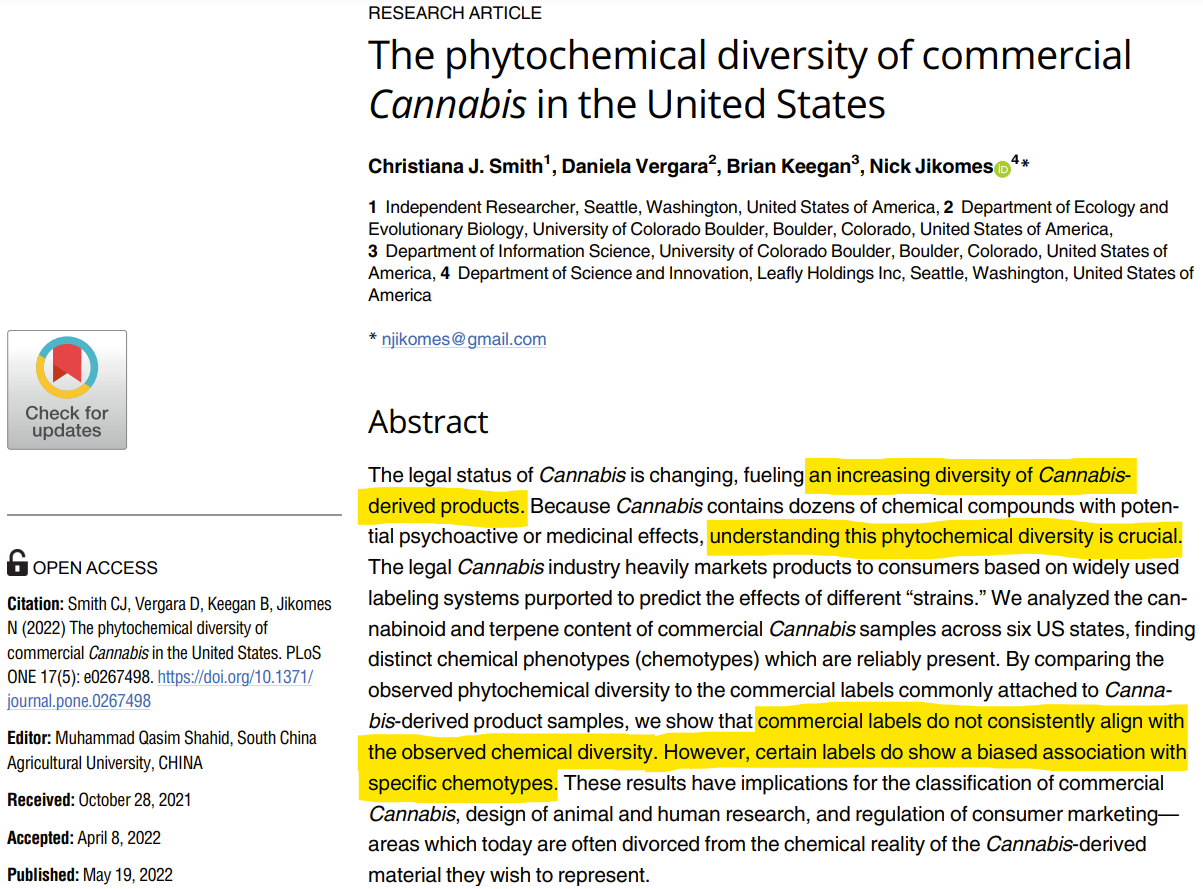
\includegraphics[width=\textwidth]{images/paper-1.png}
\end{frame}

% Paper Data
\begin{frame}{Paper Data}
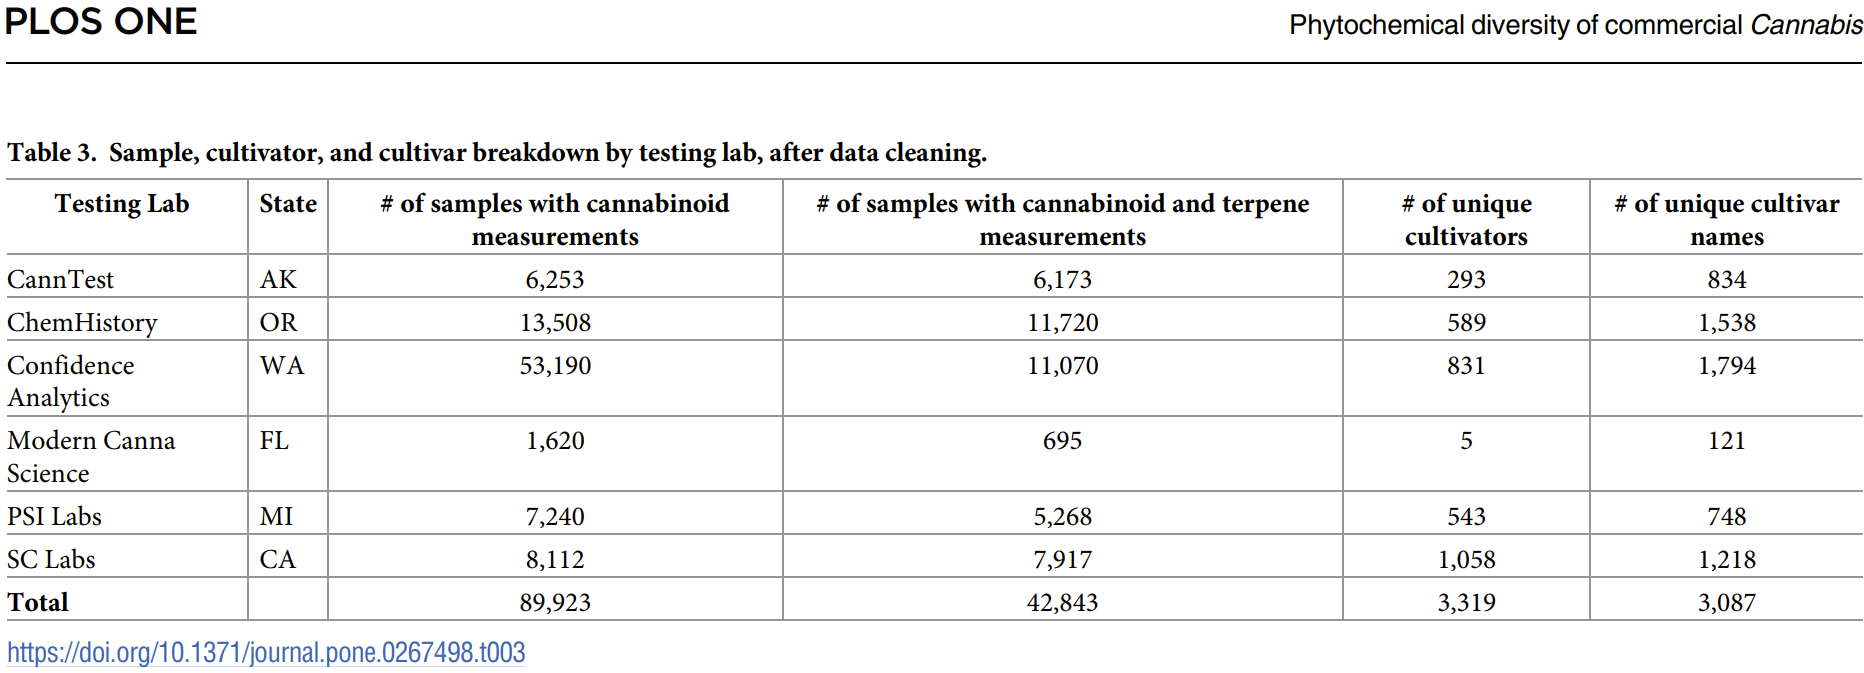
\includegraphics[width=\textwidth]{images/paper-table-1.png}
\end{frame}

% 
\begin{frame}{}
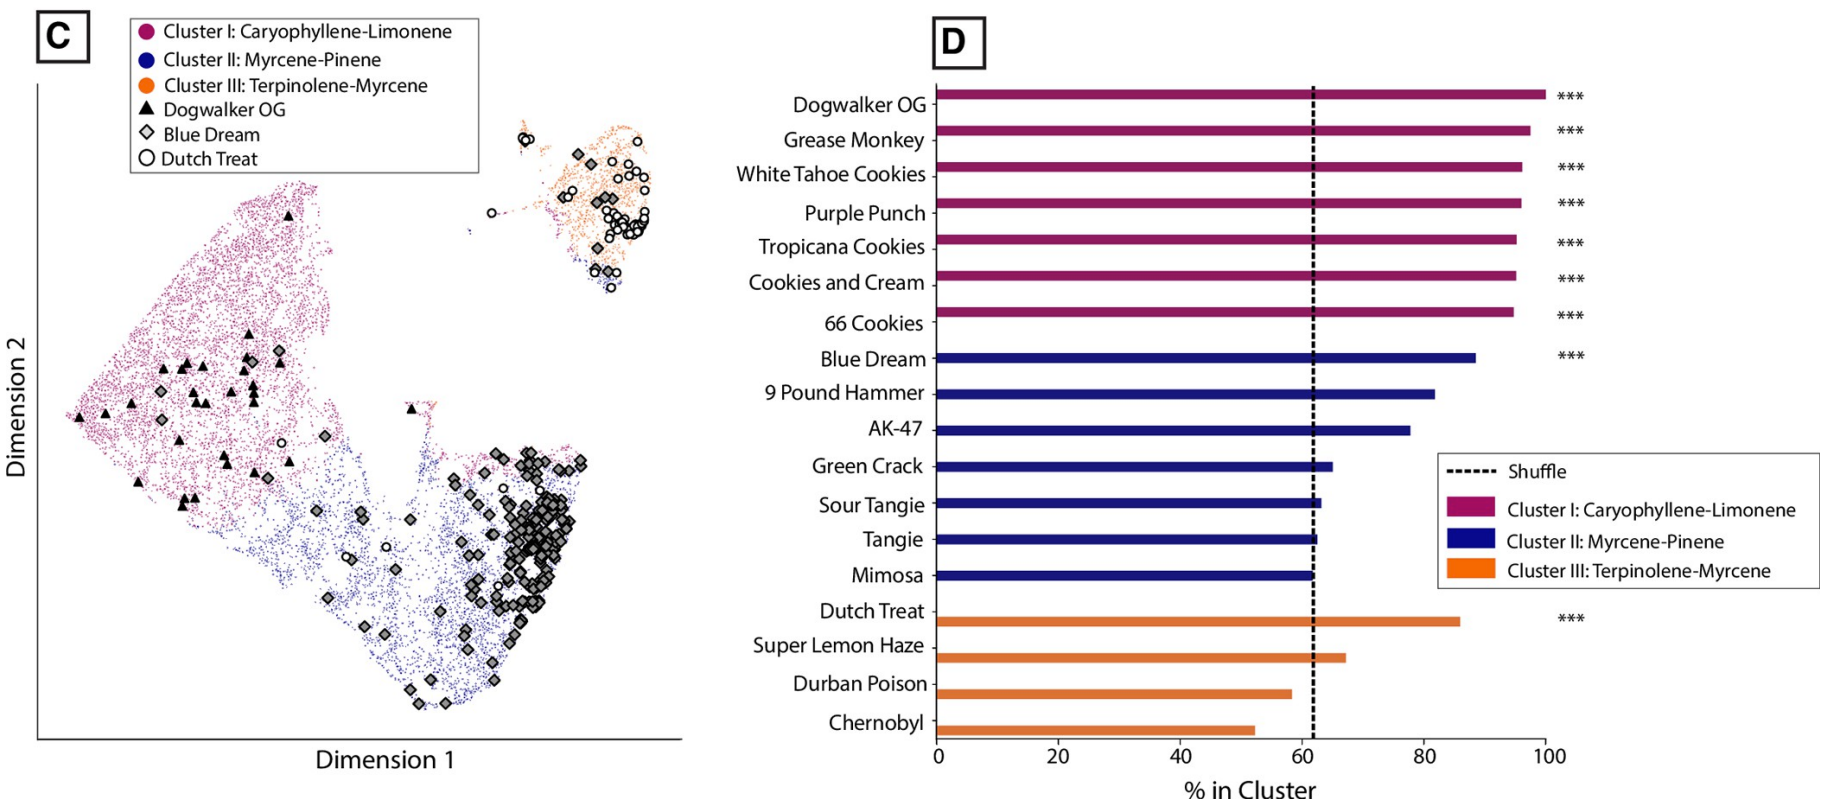
\includegraphics[width=\textwidth]{images/paper-figure-2.png}\\
\vspace{2\baselineskip}
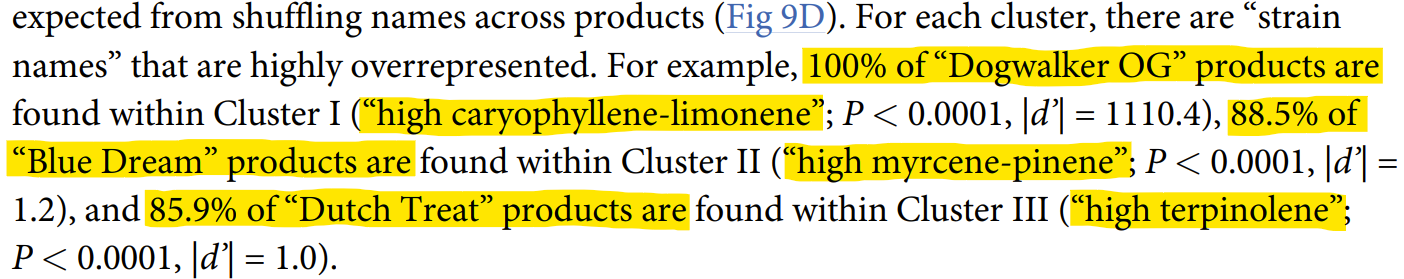
\includegraphics[width=\textwidth]{images/paper-2.png}
\end{frame}

% 
\begin{frame}{Between-Producer Cosine Similarity}
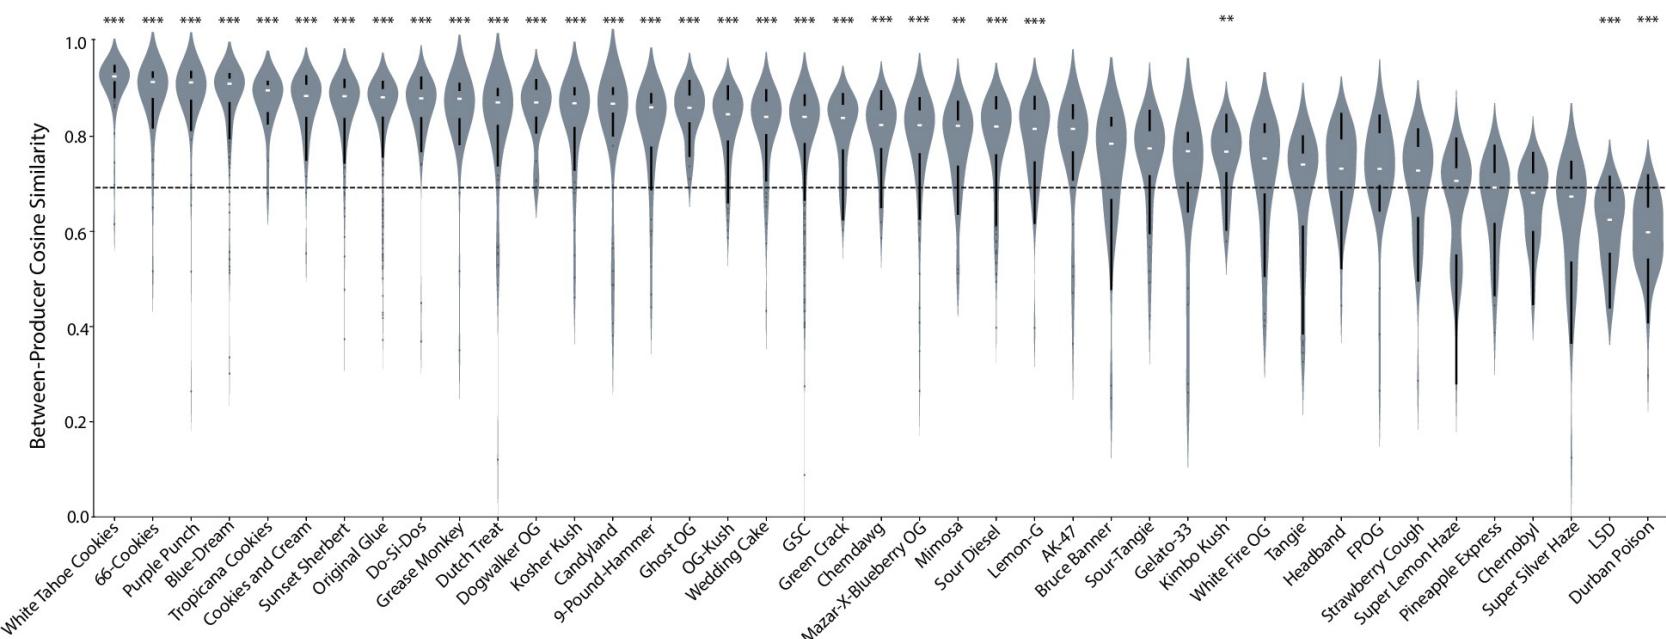
\includegraphics[width=\textwidth]{images/paper-figure-3.png}
\end{frame}

% 
\begin{frame}{}
\begin{center}
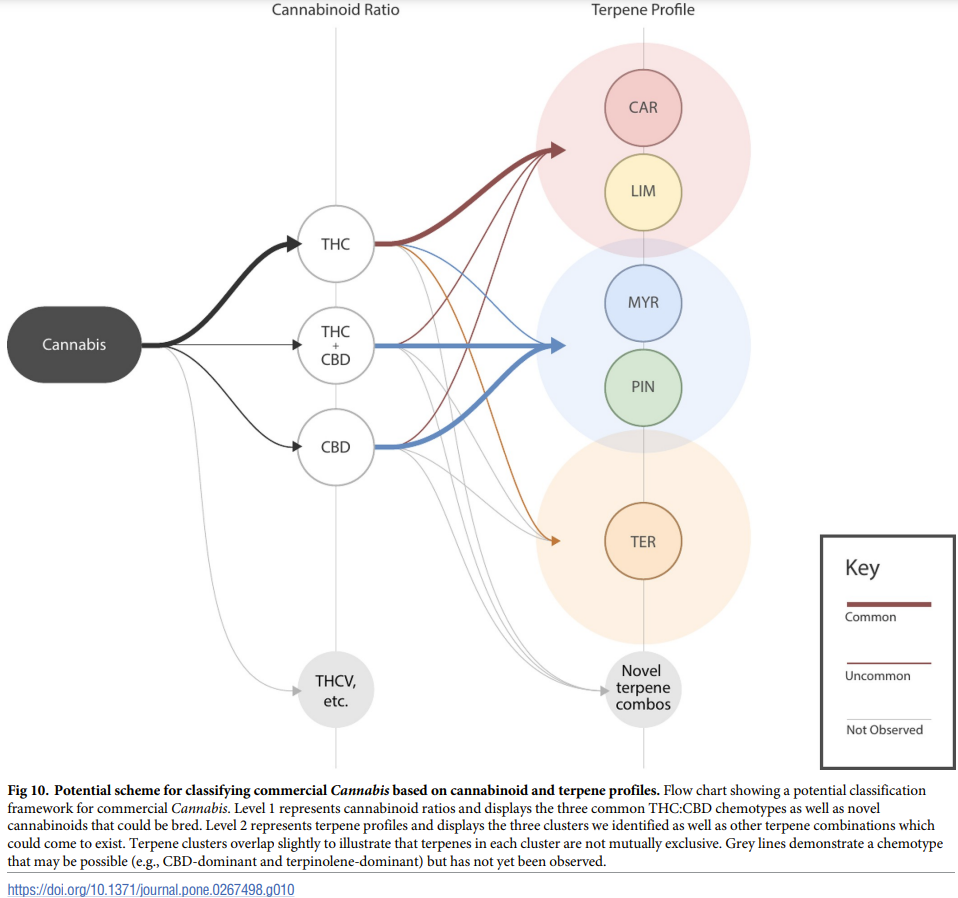
\includegraphics[width=0.9\textwidth]{images/paper-figure-1.png}
\end{center}
\end{frame}


%------------------------------------------%
% Data
%------------------------------------------%

% Our data
\begin{frame}{}

\scriptsize

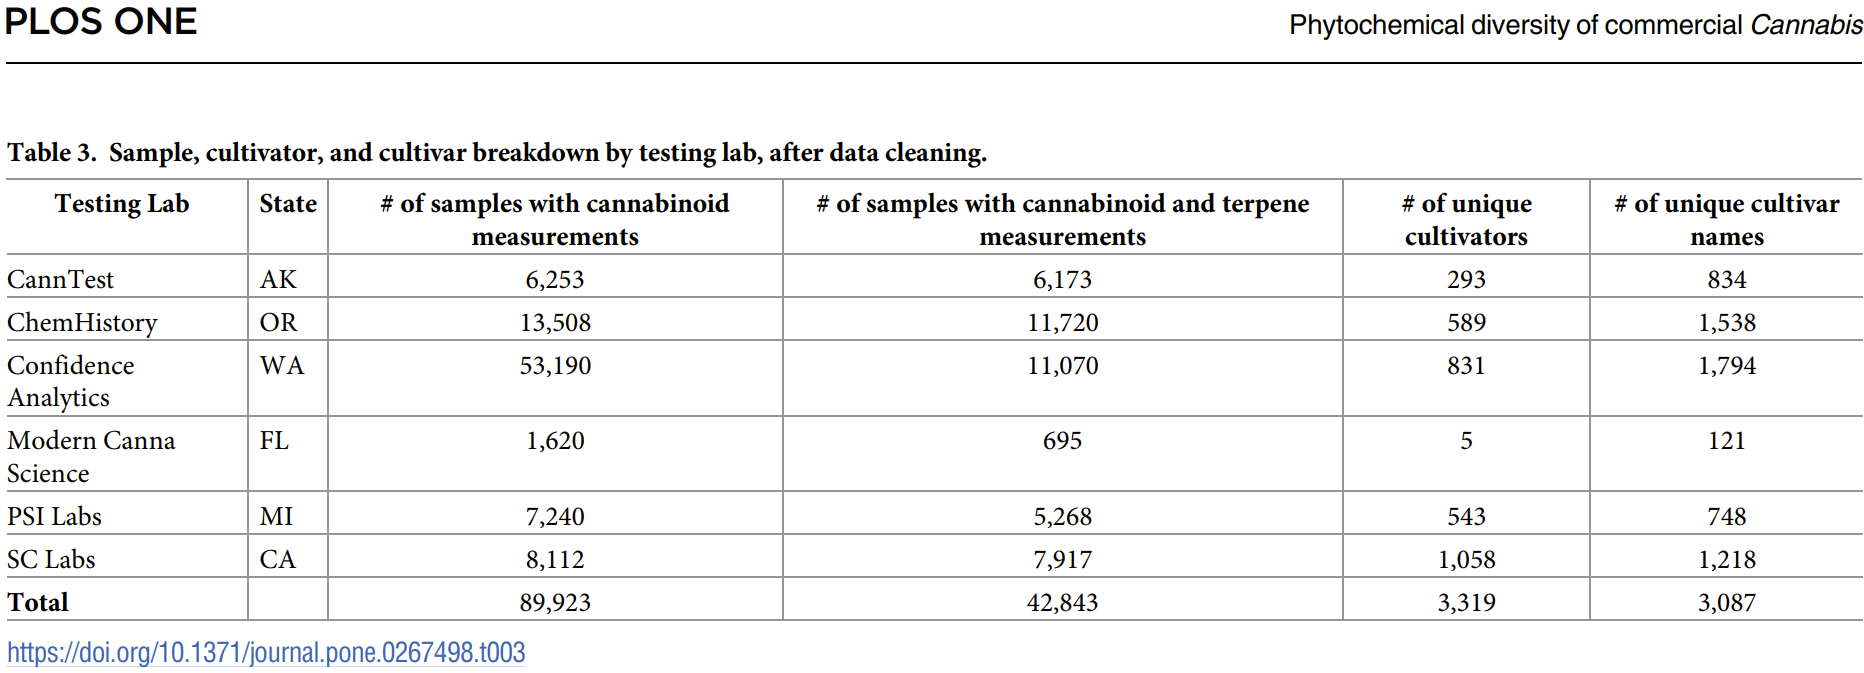
\includegraphics[width=\textwidth]{images/paper-table-1.png}\\

\vspace{1.5\baselineskip}

Lab Results Parsed from Public COAs
\vspace{0.25\baselineskip}

\begin{tabular}{lccccr}
\toprule
State & Total Tests & Flower Tests & Terpene Tests & Producers & Strains \\
\midrule
CA & 65,082 & 19,850 & 8,342 & 169 & 6,227 \\
CO & 11,031 & 5,177 & 404 & 10 & 205 \\
FL & 7,331 & 4,706 & - & - & - \\
MA & 7,189 & 3,692 & 1,950 & ? & 1,543 \\
Total & 90,633 & 33,425 & 10,696 & 179 & 7,975 \\
\bottomrule
\end{tabular}

\end{frame}

% chemical-diversity
\begin{frame}{}
\begin{center}
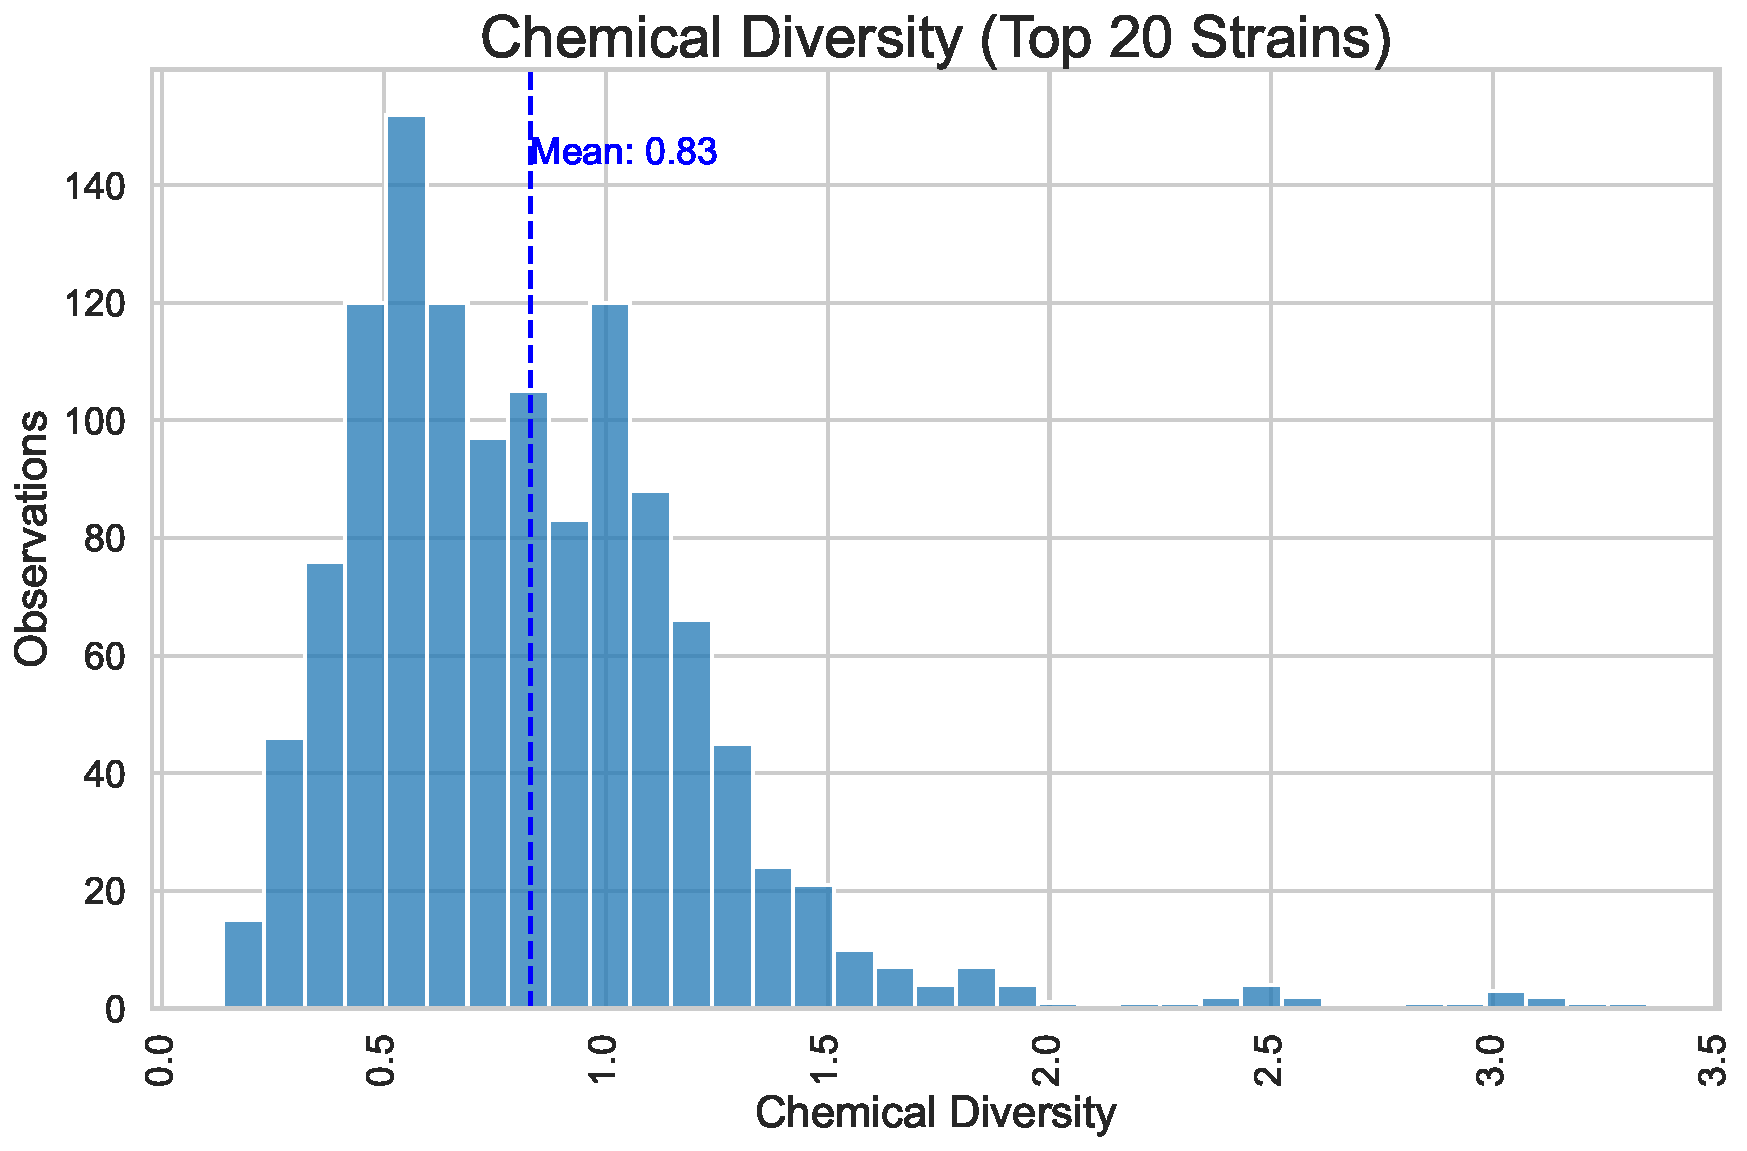
\includegraphics[width=\textwidth]{images/chemical-diversity.pdf}
\end{center}
\end{frame}

% chemical-diversity-by-month
\begin{frame}{}
\begin{center}
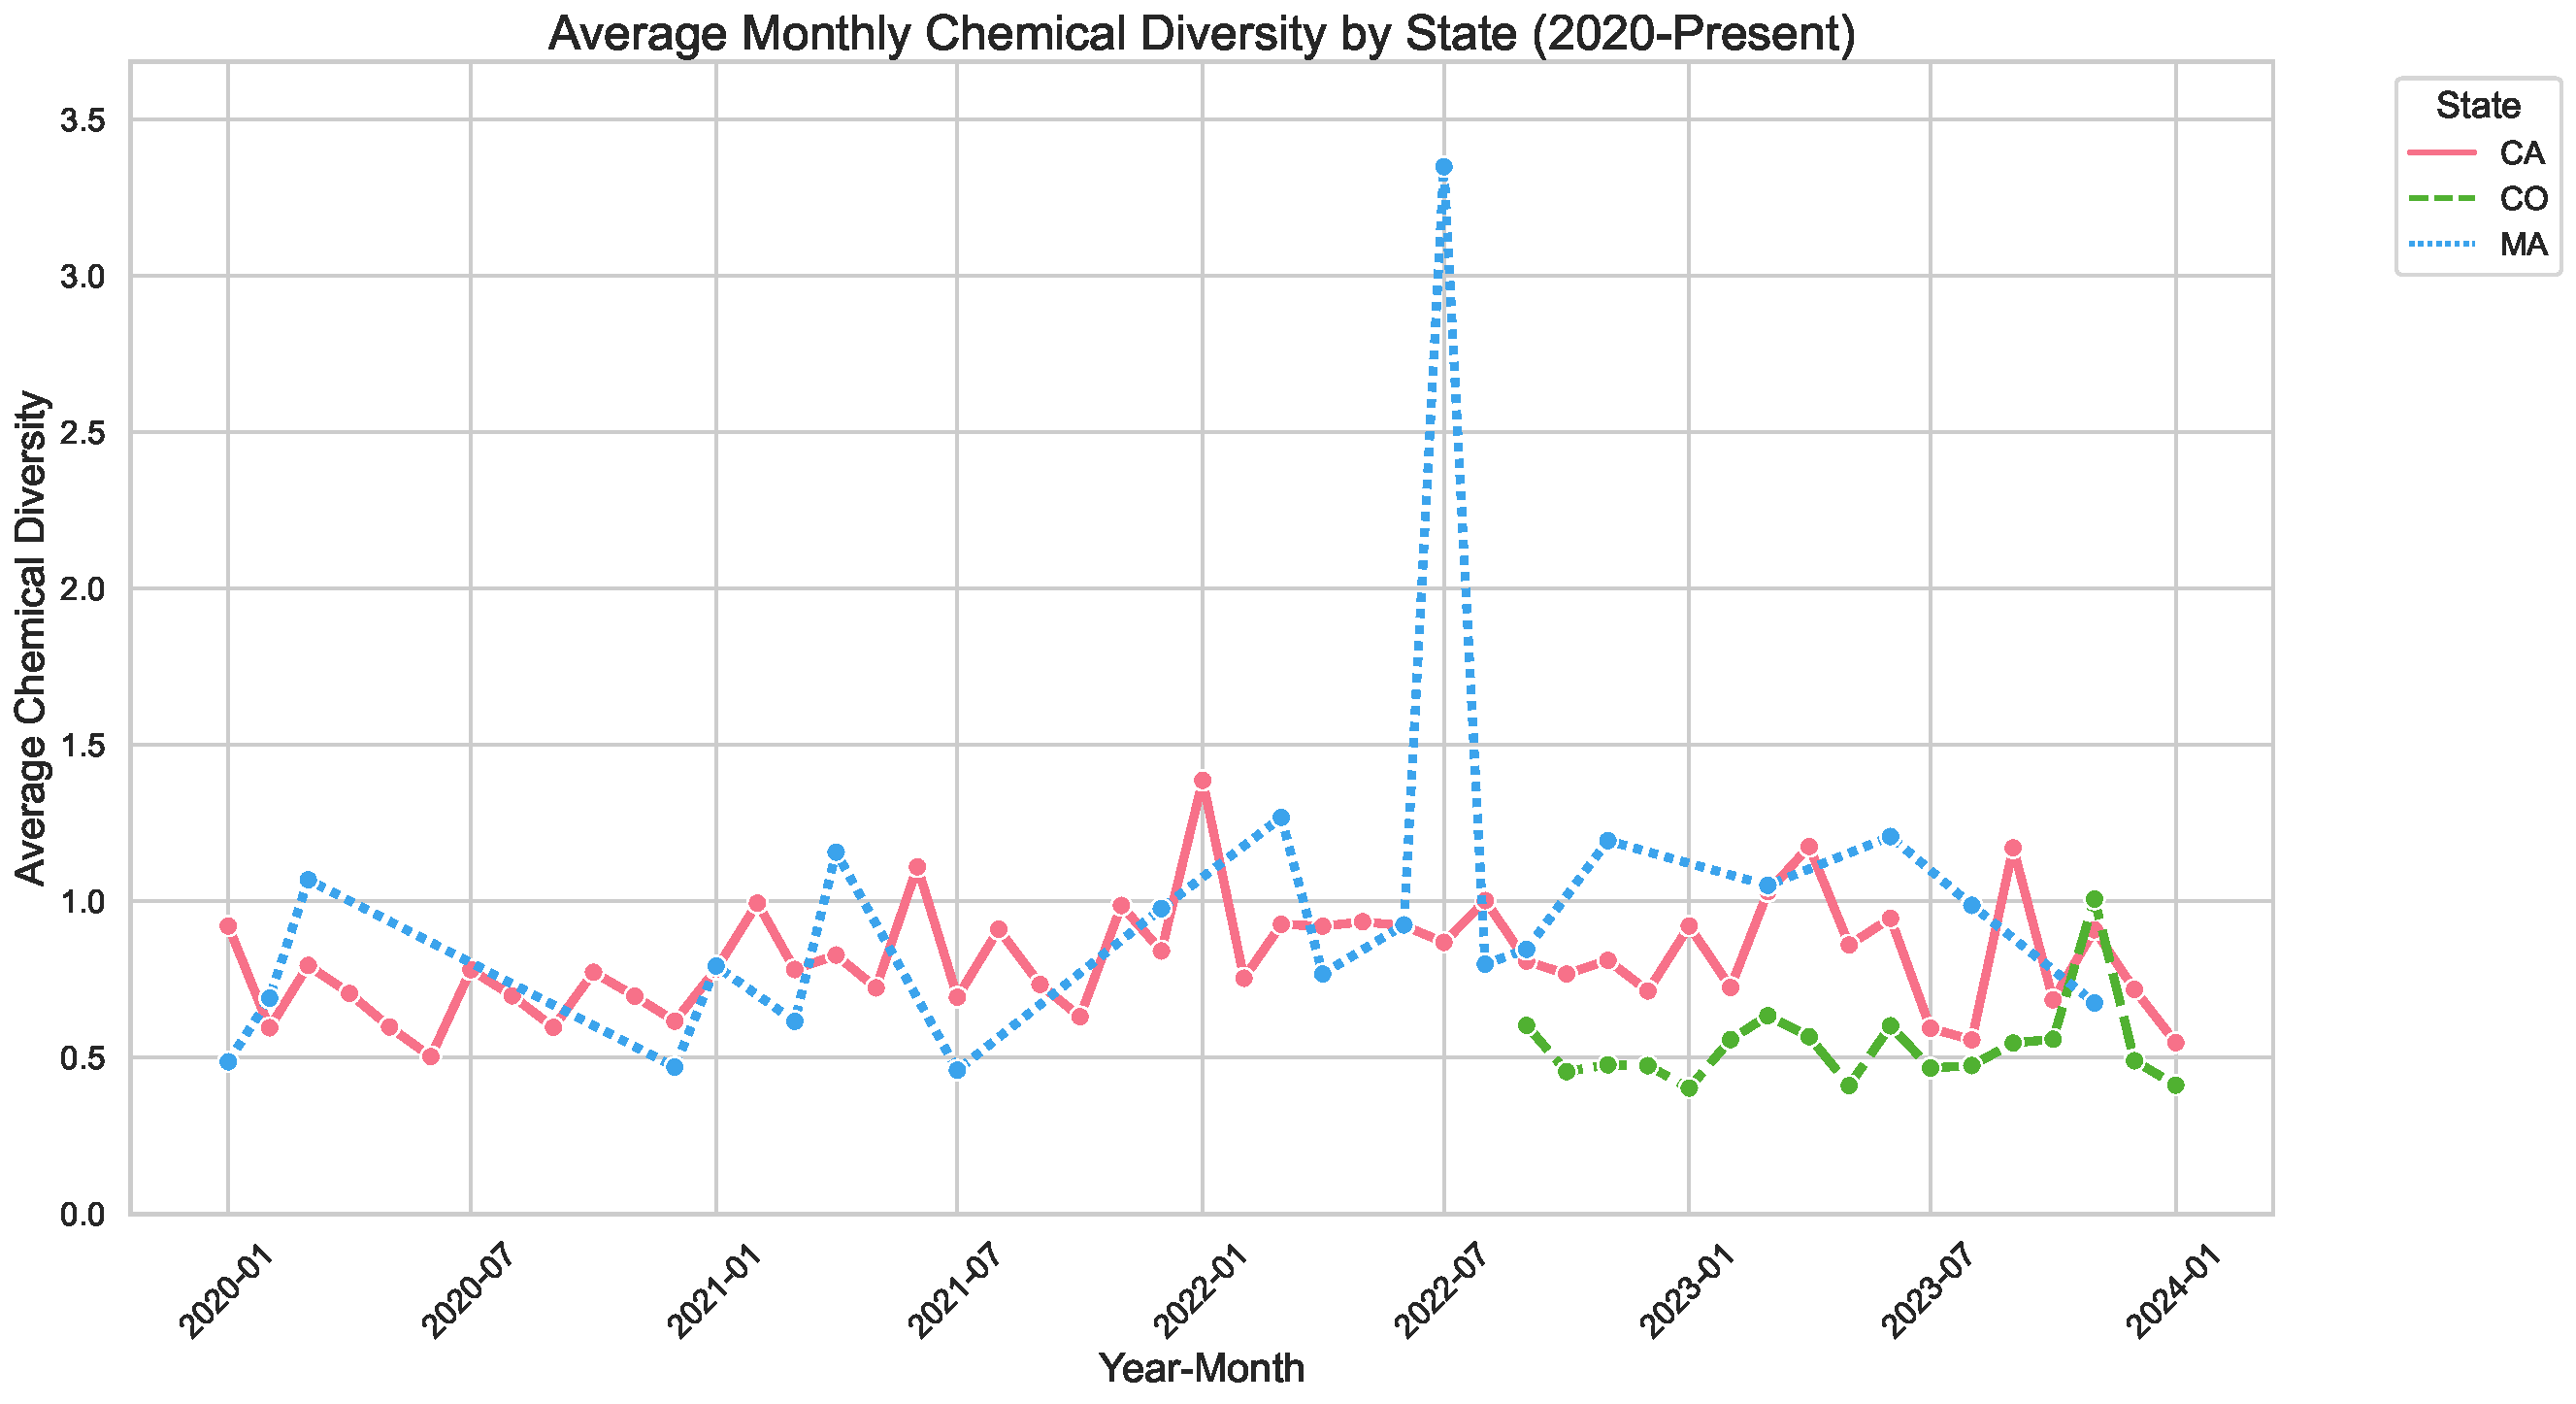
\includegraphics[width=\textwidth]{images/chemical-diversity-by-month.pdf}
\end{center}
\end{frame}

% Regression
\begin{frame}{Hypothesis 1}

\small
{\bfseries Hypothesis}: Cannabis chemical diversity is increasing over time.

\tiny

\begin{center}
\begin{tabular}{lclc}
\toprule
\textbf{Dep. Variable:}       & chemical\_diversity & \textbf{  R-squared:         } &     0.450   \\
\textbf{Model:}               &         OLS         & \textbf{  Adj. R-squared:    } &     0.434   \\
\textbf{Method:}              &    Least Squares    & \textbf{  F-statistic:       } &     28.39   \\
\textbf{Date:}                &   Thu, 25 Jan 2024  & \textbf{  Prob (F-statistic):} &  1.71e-13   \\
\textbf{Time:}                &       15:10:22      & \textbf{  Log-Likelihood:    } &   -10.071   \\
\textbf{No. Observations:}    &           108       & \textbf{  AIC:               } &     28.14   \\
\textbf{Df Residuals:}        &           104       & \textbf{  BIC:               } &     38.87   \\
\textbf{Df Model:}            &             3       & \textbf{                     } &             \\
\textbf{Covariance Type:}     &      nonrobust      & \textbf{                     } &             \\
\bottomrule
\end{tabular}
\begin{tabular}{lcccccc}
                              & \textbf{coef} & \textbf{std err} & \textbf{t} & \textbf{P$> |$t$|$} & \textbf{[0.025} & \textbf{0.975]}  \\
\midrule
\textbf{Intercept}            &       0.7038  &        0.064     &    10.948  &         0.000        &        0.576    &        0.831     \\
\textbf{C(lab\_state)[T.CO]}  &      -0.4892  &        0.083     &    -5.895  &         0.000        &       -0.654    &       -0.325     \\
\textbf{C(lab\_state)[T.MA]}  &       0.2708  &        0.057     &     4.755  &         0.000        &        0.158    &        0.384     \\
\textbf{year\_month\_numeric} &       0.0064  &        0.002     &     3.097  &         0.003        &        0.002    &        0.010     \\
\bottomrule
\end{tabular}
\end{center}


\end{frame}

% Common strains.
\begin{frame}{Common strains in the public lab results}{}

\tiny

\begin{minipage}[t]{0.45\textwidth}

Top strains mentioned in the paper
\vspace{0.25\baselineskip}

\begin{tabular}{lr}
\toprule
Strain Name & Observations \\
\midrule
Wedding Cake & 277 \\
Blue Dream & 163 \\
Sour Diesel & 128 \\
Headband & 81 \\
Mimosa & 75 \\
Tangie & 71 \\
Purple Punch & 60 \\
Green Crack & 51 \\
Kosher Kush & 47 \\
Gelato 33 & 41 \\
Chemdawg & 34 \\
Grease Monkey & 32 \\
Pineapple Express & 27 \\
Super Lemon Haze & 26 \\
Lemon G & 26 \\
Durban Poison & 25 \\
Strawberry Cough & 21 \\
Sunset Sherbert & 18 \\
Sour Tangie & 15 \\
Chernobyl & 15 \\
\bottomrule
\end{tabular}

\end{minipage}%
\begin{minipage}[t]{0.45\textwidth}

Top strains in the pubic lab results
\vspace{0.25\baselineskip}

\begin{tabular}{lr}
\toprule
Strain Name & Observations \\
\midrule
Gelato & 715 \\
Runtz & 462 \\
Wedding Cake & 278 \\
GMO & 194 \\
Blue Dream & 163 \\
GG4 & 96 \\
Zkittles & 72 \\
OG Kush & 70 \\
White Truffle & 42 \\
Dolato & 27 \\
Skywalker OG & 21 \\
Strawberry Cough & 21 \\
\bottomrule
\end{tabular}

\end{minipage}

\end{frame}

% TODO: Elevation and plant hardiness zone data.
% https://planthardiness.ars.usda.gov/
% https://www.opentopodata.org/


%------------------------------------------%
% Analysis
%------------------------------------------%

% terpenes-by-strain
\begin{frame}{}
\begin{center}
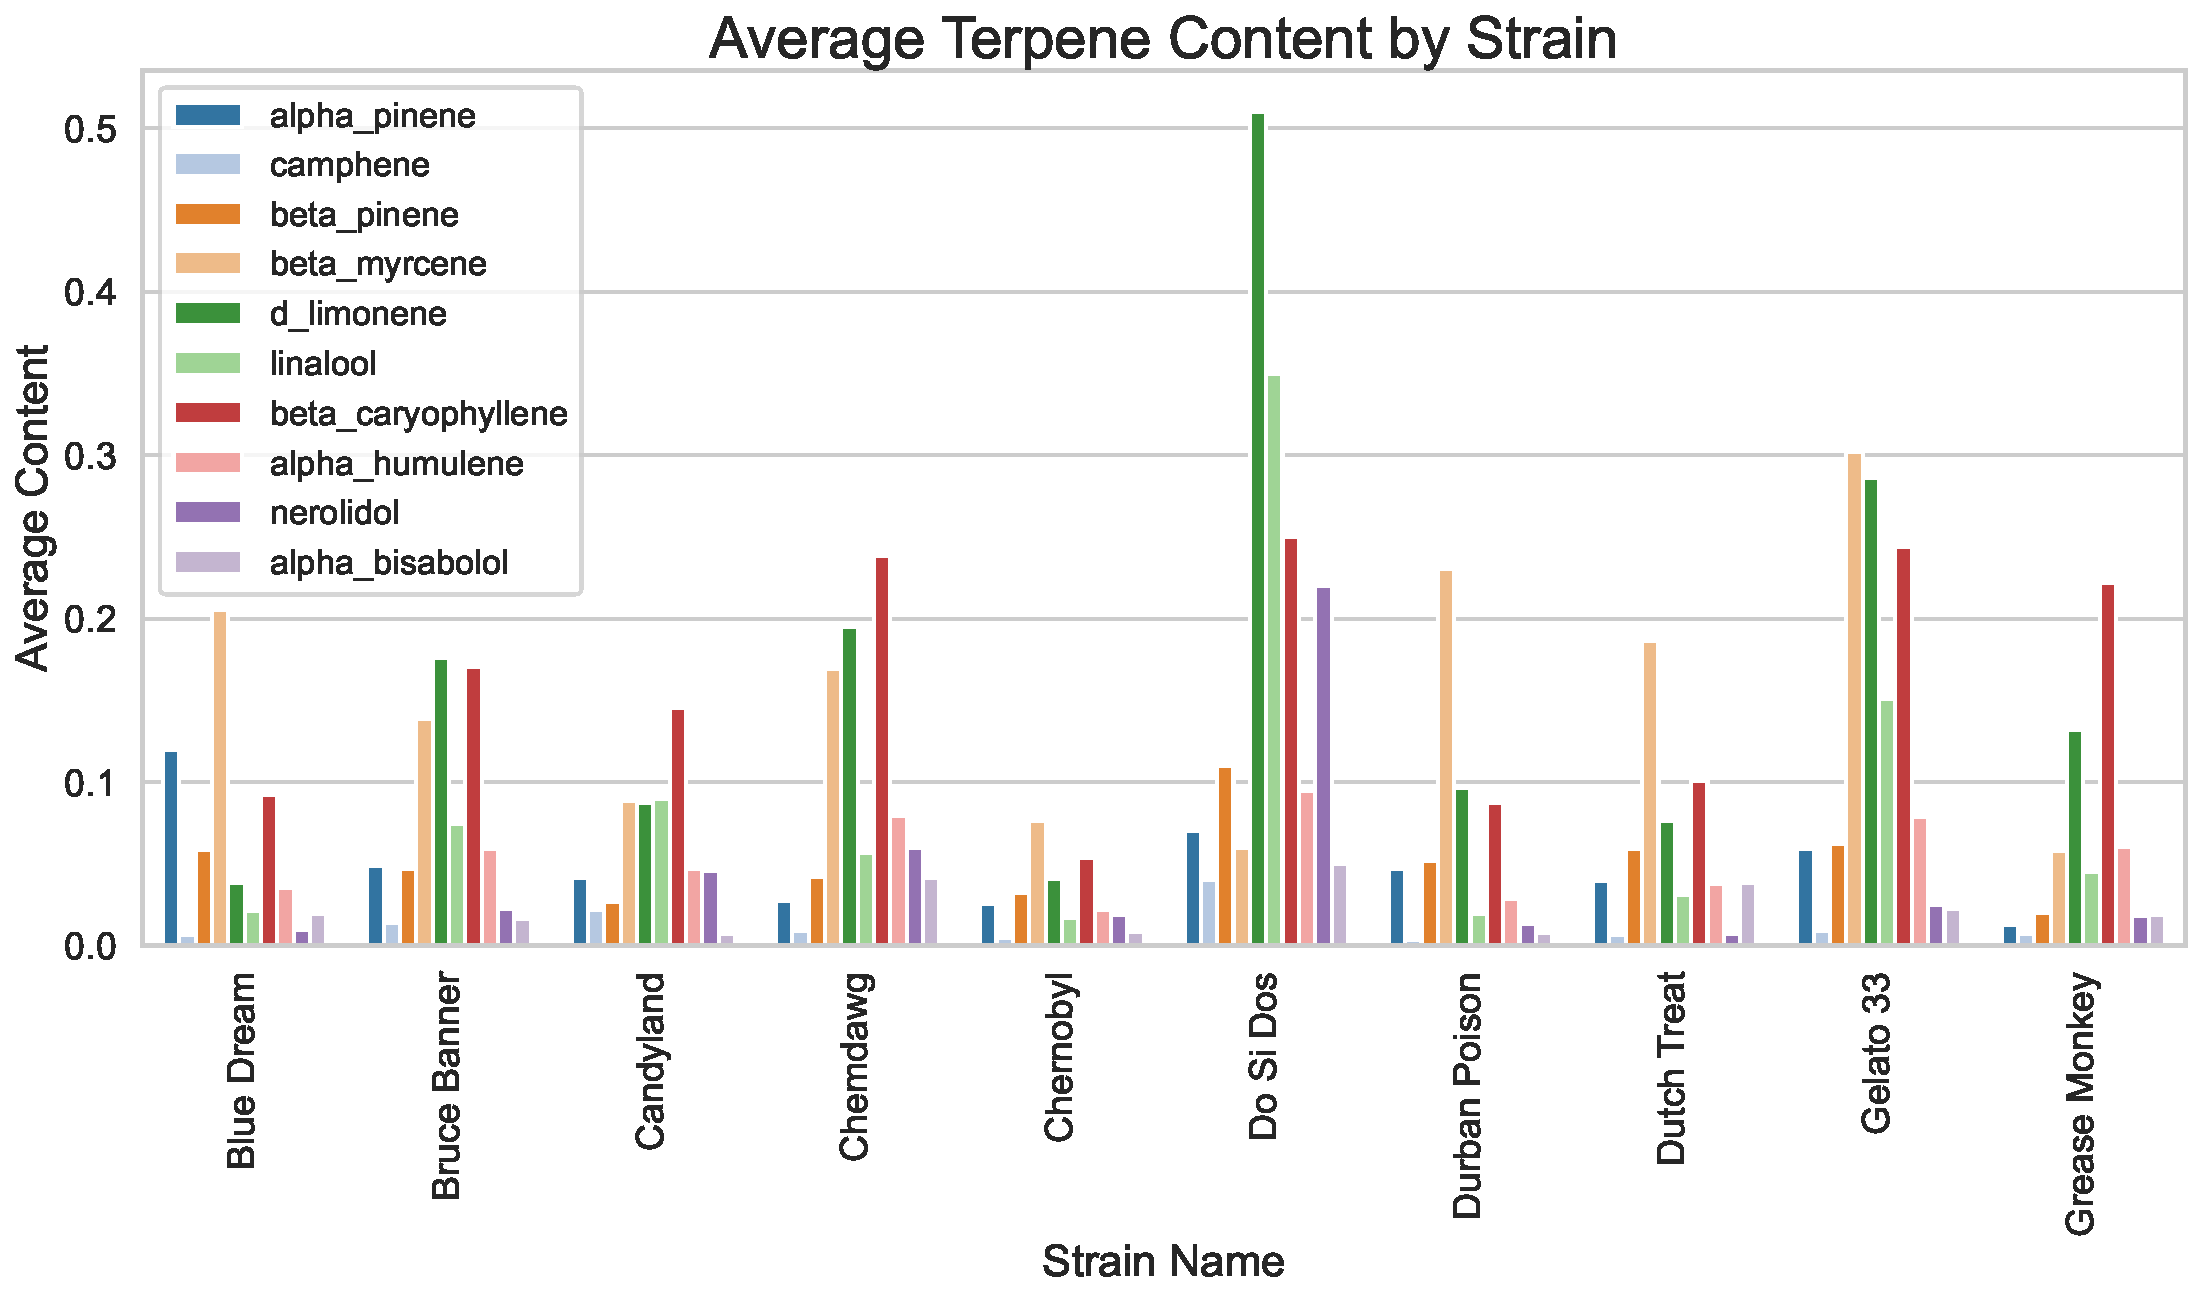
\includegraphics[width=\textwidth]{images/terpenes-by-strain.pdf}
\end{center}
\end{frame}

% caryophyllene-limonene
\begin{frame}{}
\begin{center}
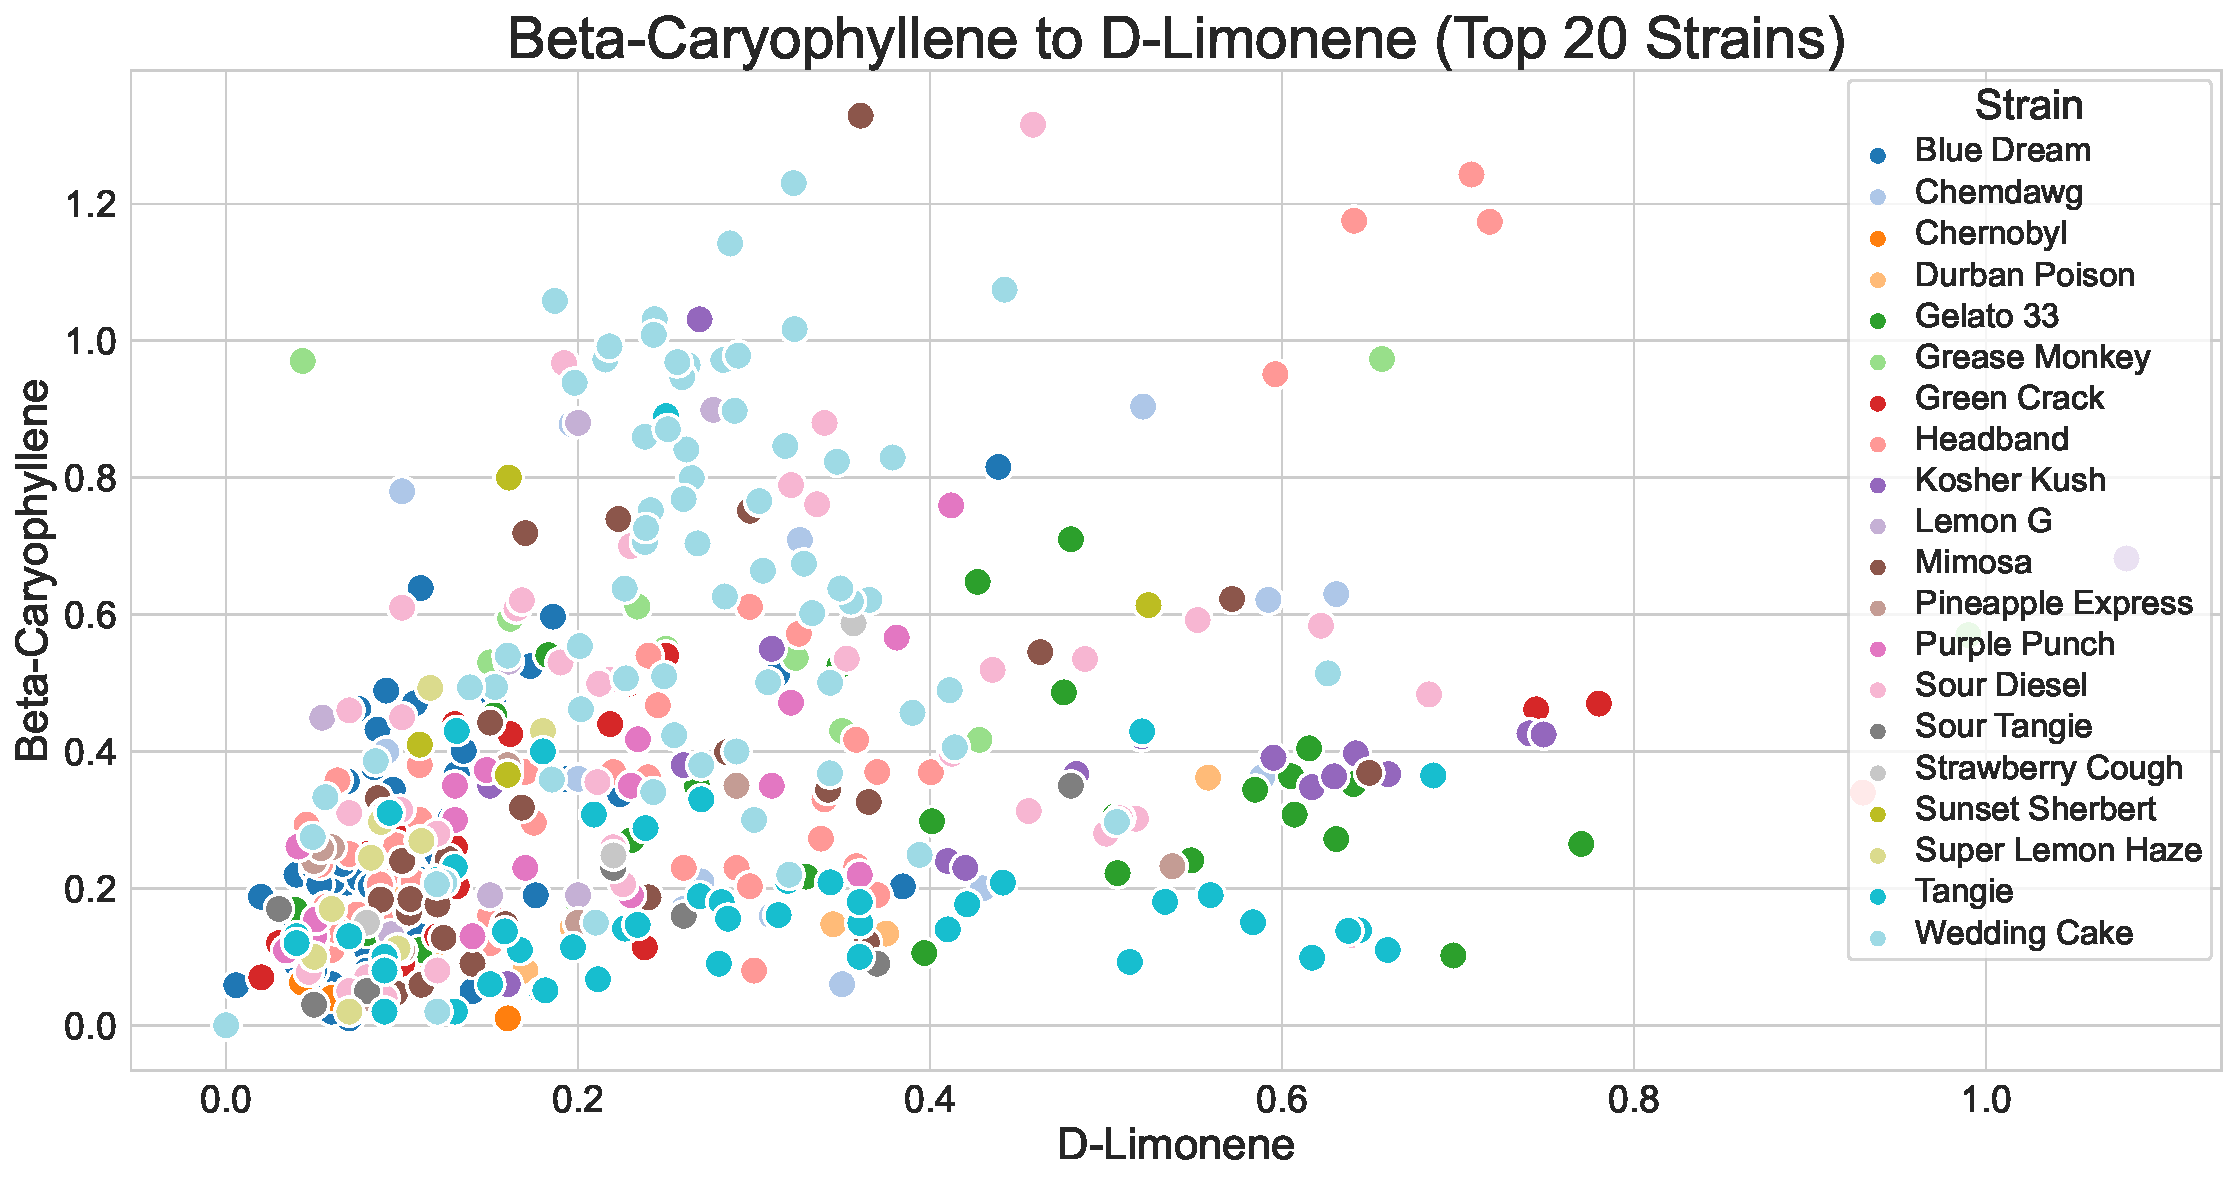
\includegraphics[width=\textwidth]{images/top-20-caryophyllene-limonene.pdf}
\end{center}
\end{frame}

% myrcene-pinene
\begin{frame}{}
\begin{center}
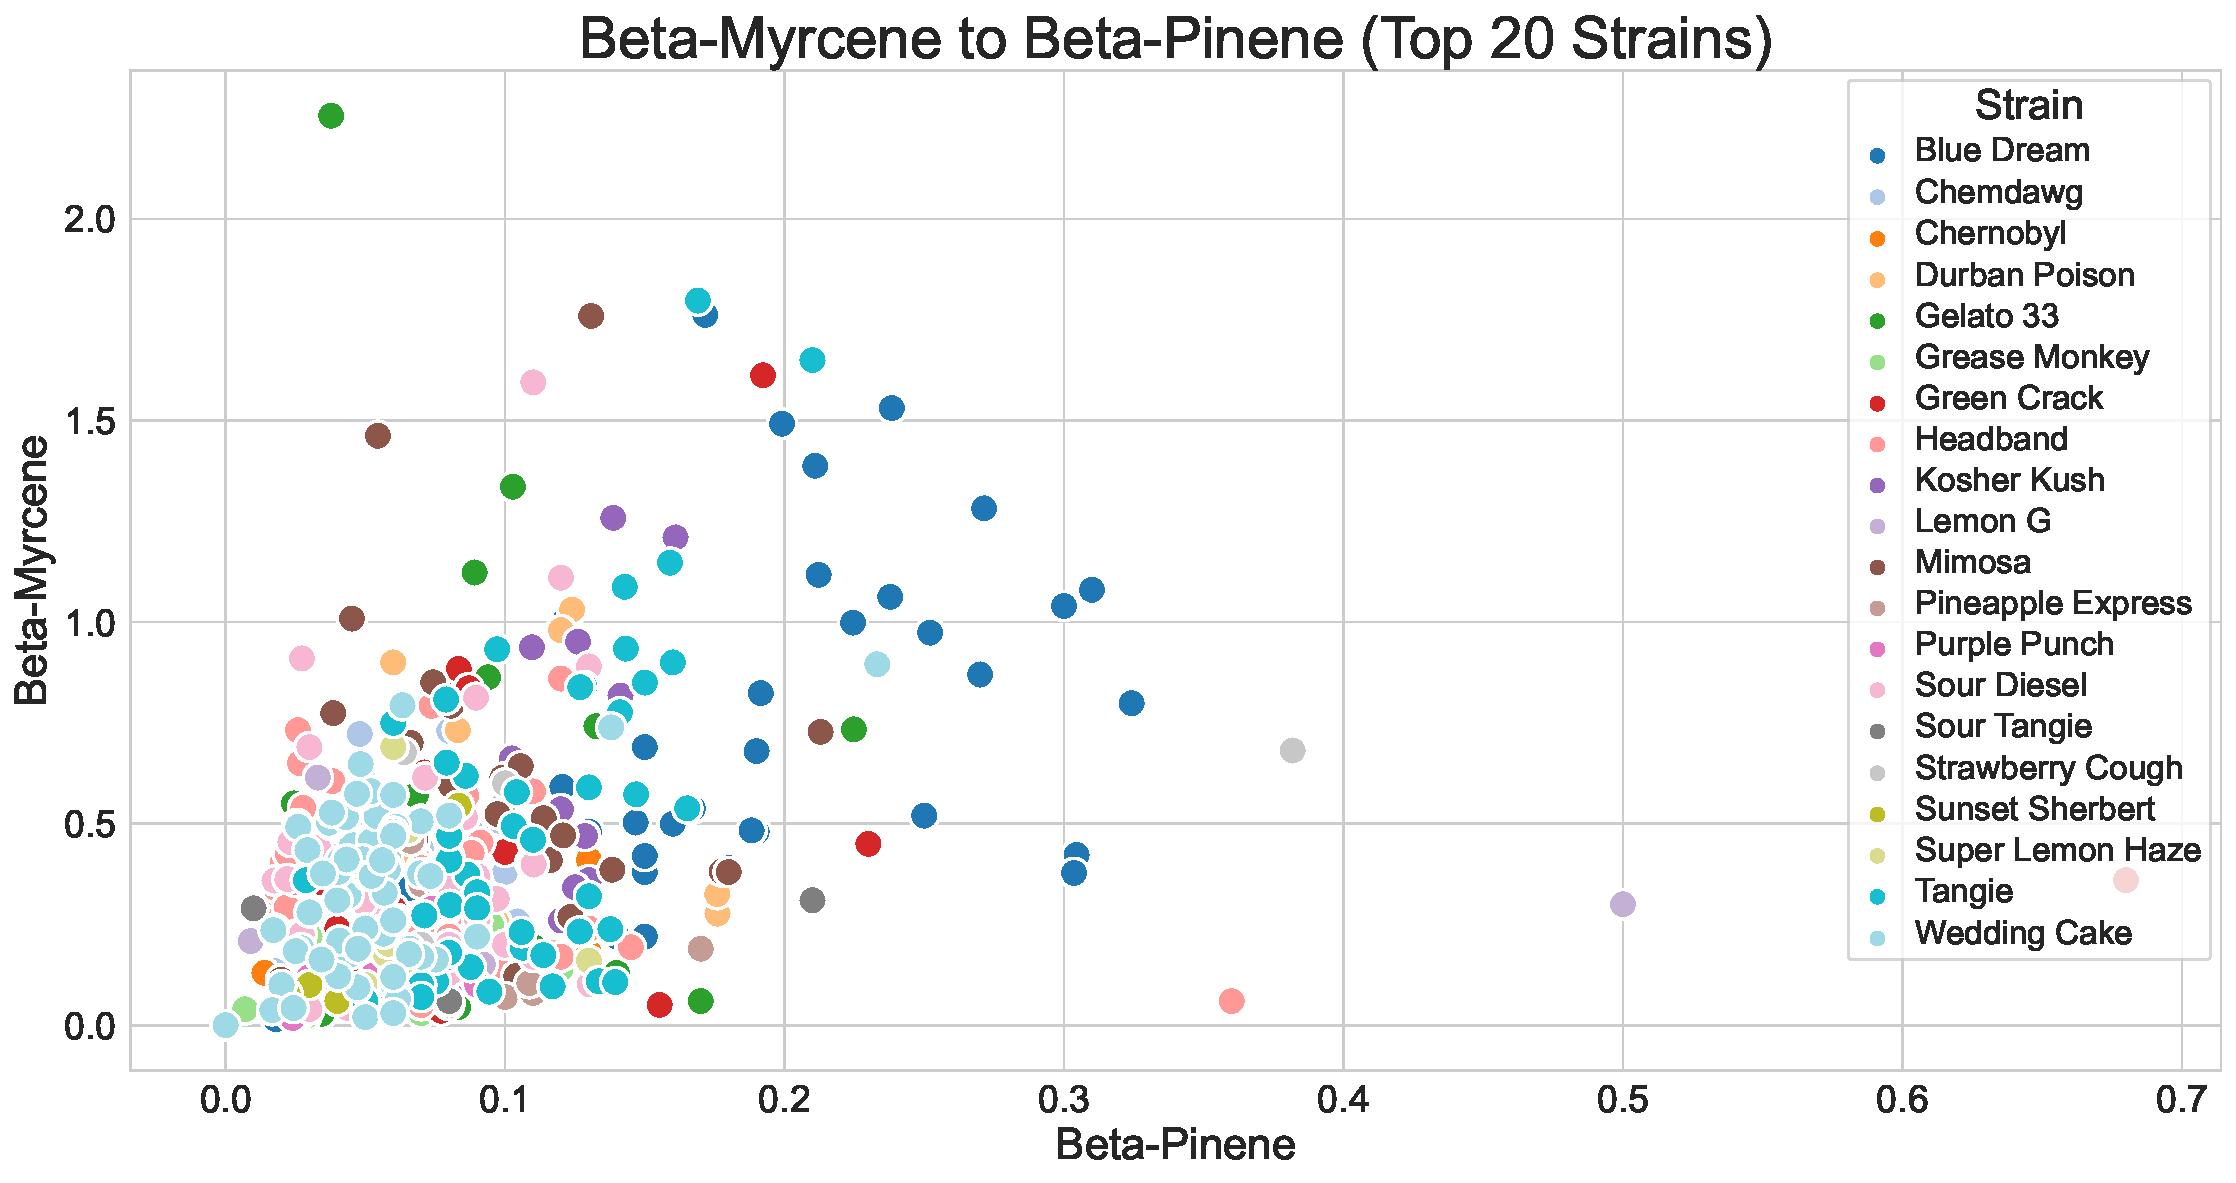
\includegraphics[width=\textwidth]{images/top-20-myrcene-pinene.pdf}
\end{center}
\end{frame}

% Beta-pinene to D-limonene
\begin{frame}{}
\begin{center}
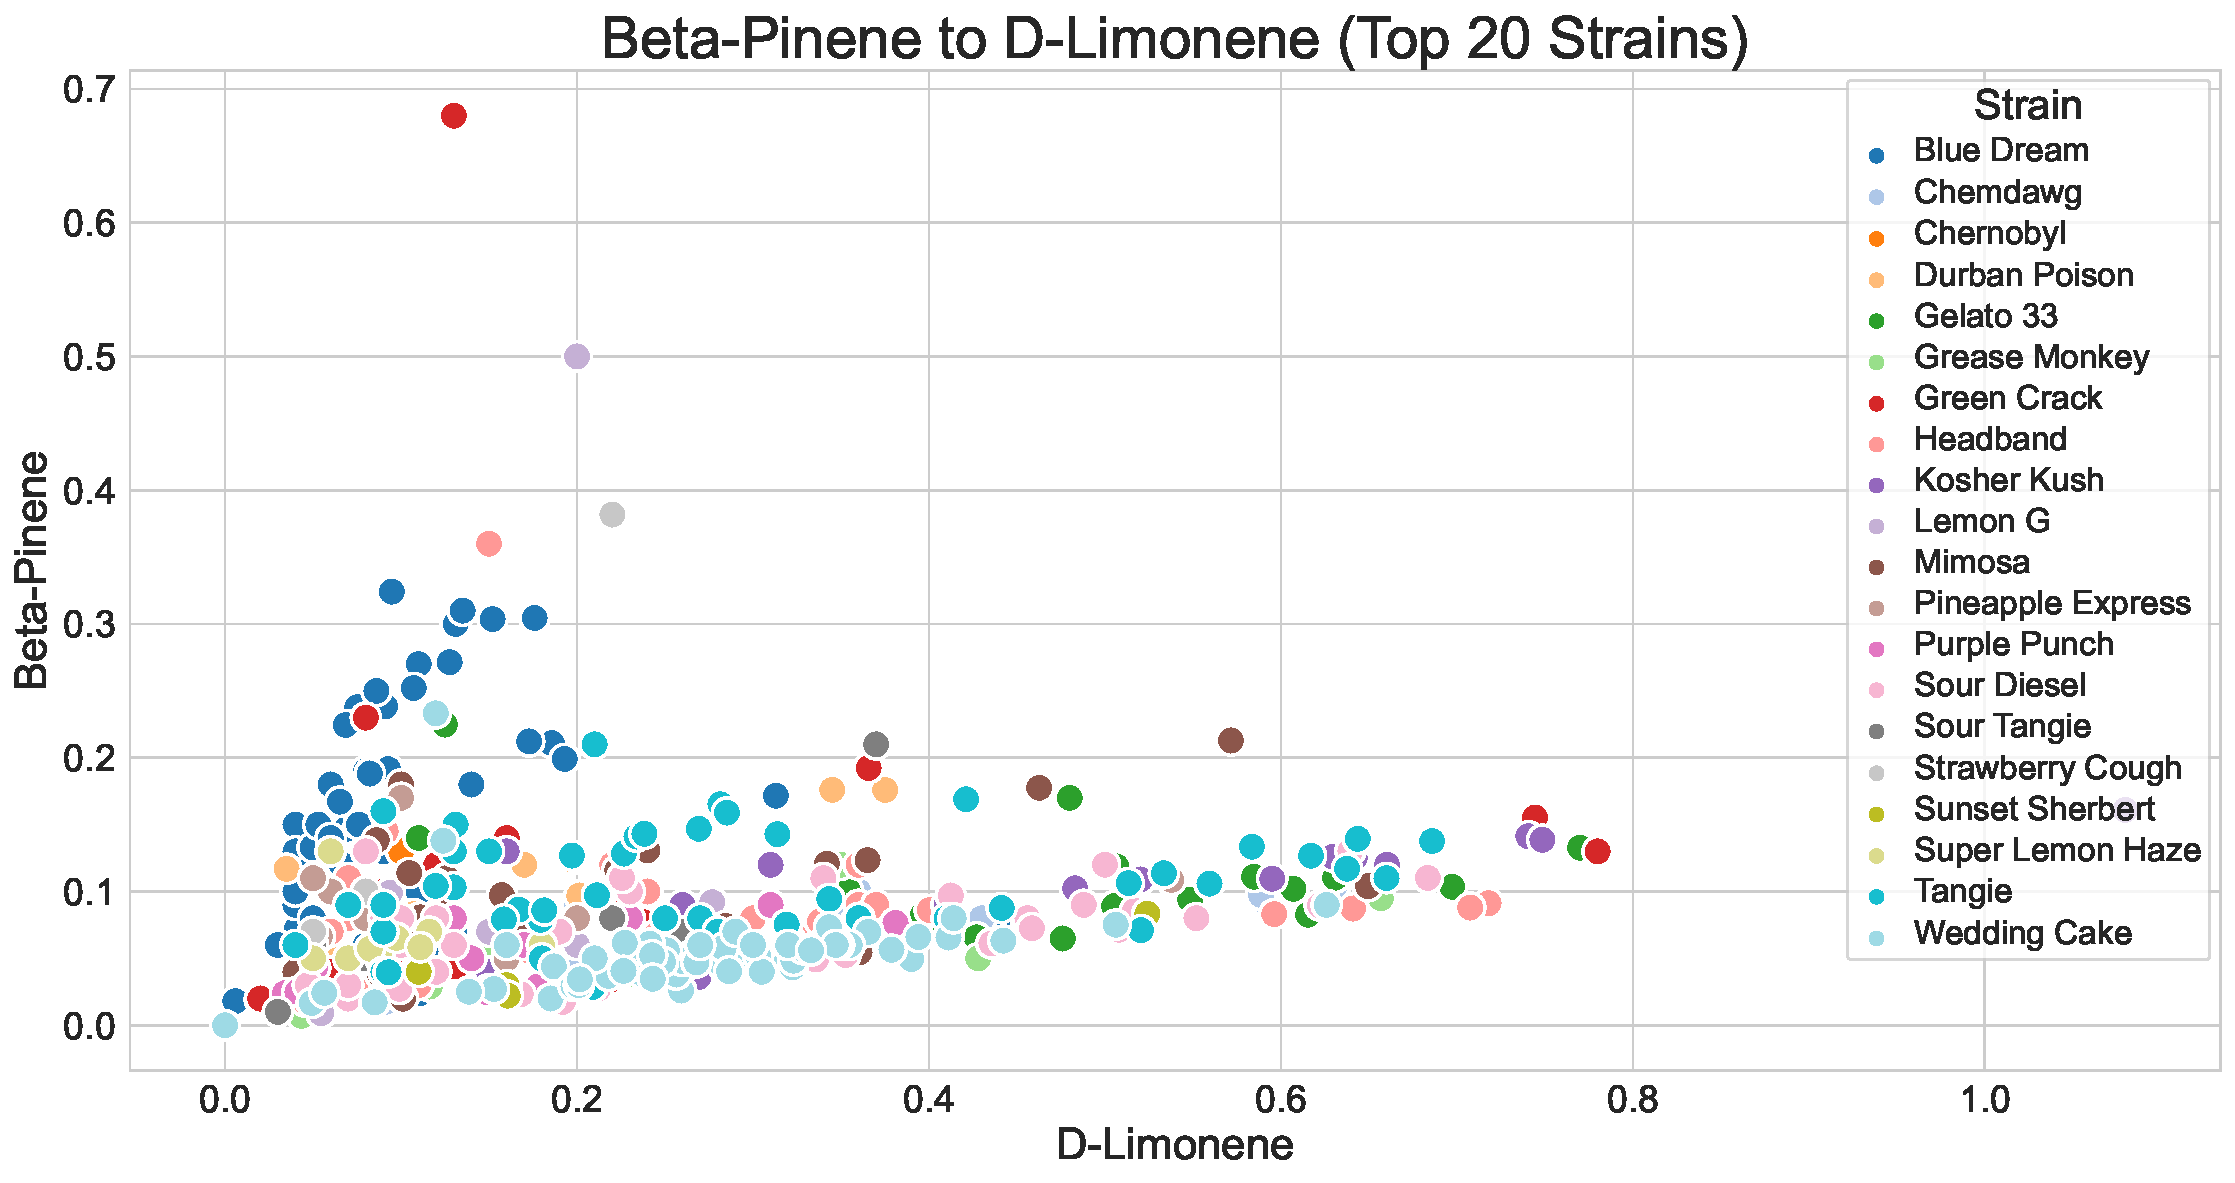
\includegraphics[width=\textwidth]{images/top-20-pinene-limonene.pdf}
\end{center}
\end{frame}

% Hypothesis 2
\begin{frame}{Hypothesis 2}

\small
{\bfseries Hypothesis}: "Blue Dream" strains have higher beta-pinene than other top strains, on average.

\tiny
\begin{center}
\begin{tabular}{lclc}
\toprule
\textbf{Dep. Variable:}    &   beta\_pinene   & \textbf{  R-squared:         } &     0.021   \\
\textbf{Model:}            &       OLS        & \textbf{  Adj. R-squared:    } &     0.021   \\
\textbf{Method:}           &  Least Squares   & \textbf{  F-statistic:       } &     28.03   \\
\textbf{Date:}             & Thu, 25 Jan 2024 & \textbf{  Prob (F-statistic):} &  1.40e-07   \\
\textbf{Time:}             &     15:14:07     & \textbf{  Log-Likelihood:    } &    1828.4   \\
\textbf{No. Observations:} &        1288      & \textbf{  AIC:               } &    -3653.   \\
\textbf{Df Residuals:}     &        1286      & \textbf{  BIC:               } &    -3643.   \\
\textbf{Df Model:}         &           1      & \textbf{                     } &             \\
\textbf{Covariance Type:}  &    nonrobust     & \textbf{                     } &             \\
\bottomrule
\end{tabular}
\begin{tabular}{lcccccc}
                         & \textbf{coef} & \textbf{std err} & \textbf{t} & \textbf{P$> |$t$|$} & \textbf{[0.025} & \textbf{0.975]}  \\
\midrule
\textbf{const}           &       0.0326  &        0.002     &    18.647  &         0.000        &        0.029    &        0.036     \\
\textbf{is\_blue\_dream} &       0.0260  &        0.005     &     5.294  &         0.000        &        0.016    &        0.036     \\
\bottomrule
\end{tabular}
\end{center}

\end{frame}

% terpenes-by-state
\begin{frame}{}
\begin{center}
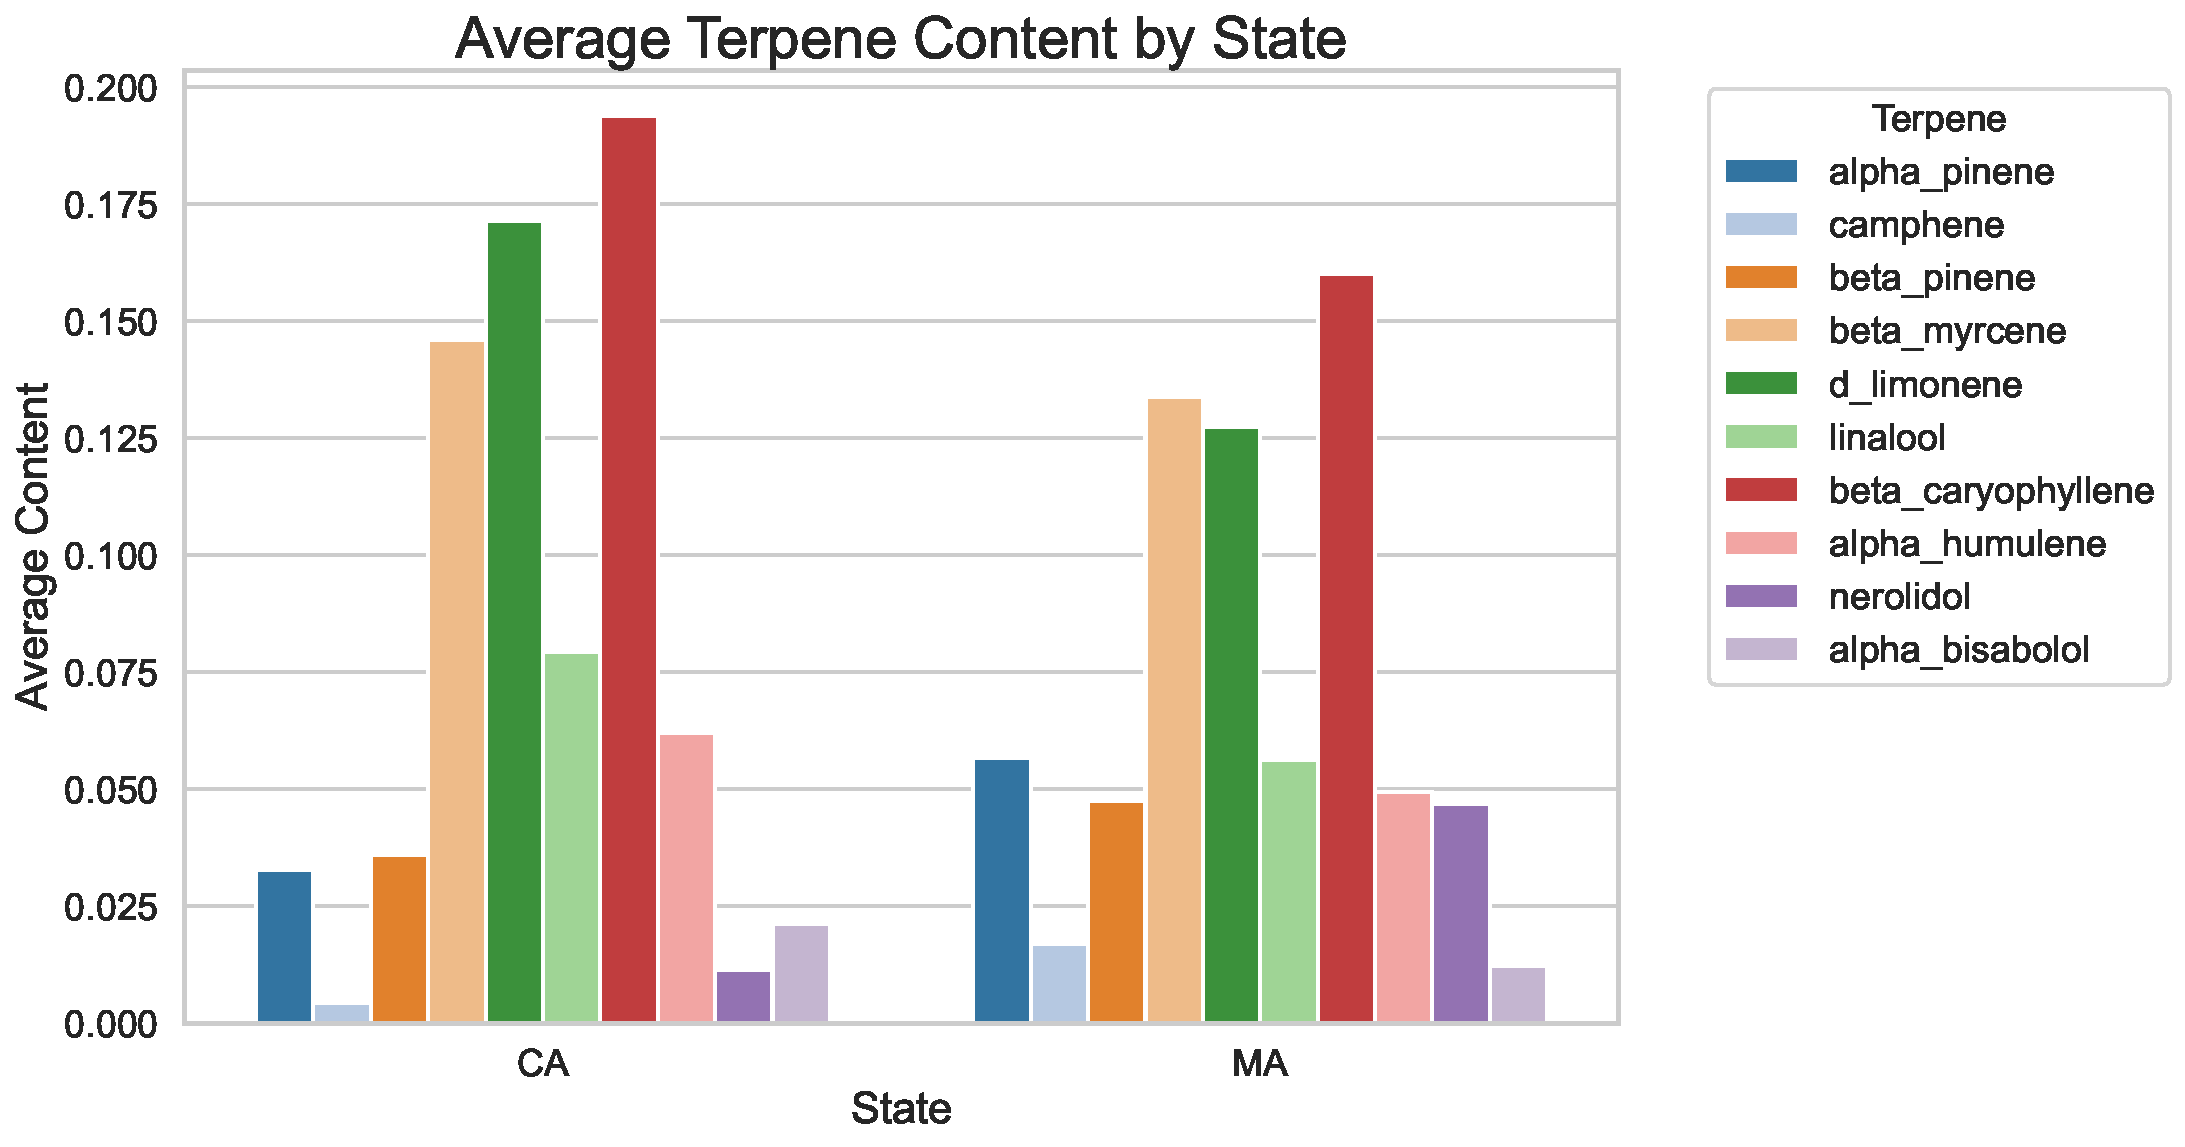
\includegraphics[width=\textwidth]{images/terpenes-by-state.pdf}
\end{center}
\end{frame}


% Chemical diversity by geography
\begin{frame}{}

\tiny

Lab results by county (for the top 20 strains)
\vspace{0.25\baselineskip}

\begin{tabular}{lr}
\toprule
County & Observations \\
\midrule
Denver County & 121 \\
Humboldt County & 56 \\
Mendocino County & 48 \\
Los Angeles County & 42 \\
Sacramento County & 38 \\
Sonoma County & 23 \\
Monterey County & 20 \\
Santa Barbara County & 19 \\
Alameda County & 14 \\
Lake County & 13 \\
El Paso County & 13 \\
Larimer County & 11 \\
San Francisco County & 8 \\
Trinity County & 7 \\
Riverside County & 7 \\
Santa Cruz County & 6 \\
Huerfano County & 5 \\
San Bernardino County & 4 \\
Routt County & 4 \\
Yolo County & 4 \\
\bottomrule
\end{tabular}

\end{frame}

% Hypothesis 3
\begin{frame}{Hypothesis 3}

\small
{\bfseries Hypothesis}: "Emerald Triangle" counties, Humboldt, Mendocino, and Trinity, produce cannabis with higher terpene concentrations than cannabis produced in other counties, on average.

\tiny
\begin{center}
\begin{tabular}{lclc}
\toprule
\textbf{Dep. Variable:}                & total\_terpenes  & \textbf{  R-squared:         } &     0.046   \\
\textbf{Model:}                        &       OLS        & \textbf{  Adj. R-squared:    } &     0.046   \\
\textbf{Method:}                       &  Least Squares   & \textbf{  F-statistic:       } &     1622.   \\
\textbf{Date:}                         & Thu, 25 Jan 2024 & \textbf{  Prob (F-statistic):} &     0.00    \\
\textbf{Time:}                         &     15:16:06     & \textbf{  Log-Likelihood:    } &   -44550.   \\
\textbf{No. Observations:}             &       33425      & \textbf{  AIC:               } & 8.910e+04   \\
\textbf{Df Residuals:}                 &       33423      & \textbf{  BIC:               } & 8.912e+04   \\
\textbf{Df Model:}                     &           1      & \textbf{                     } &             \\
\textbf{Covariance Type:}              &    nonrobust     & \textbf{                     } &             \\
\bottomrule
\end{tabular}
\begin{tabular}{lcccccc}
                                       & \textbf{coef} & \textbf{std err} & \textbf{t} & \textbf{P$> |$t$|$} & \textbf{[0.025} & \textbf{0.975]}  \\
\midrule
\textbf{Intercept}                     &       0.5267  &        0.005     &   101.567  &         0.000        &        0.517    &        0.537     \\
\textbf{C(is\_emerald\_triangle)[T.1]} &       0.8297  &        0.021     &    40.276  &         0.000        &        0.789    &        0.870     \\
\bottomrule
\end{tabular}
\end{center}

\end{frame}

% terpenes-by-month
\begin{frame}{}
\begin{center}
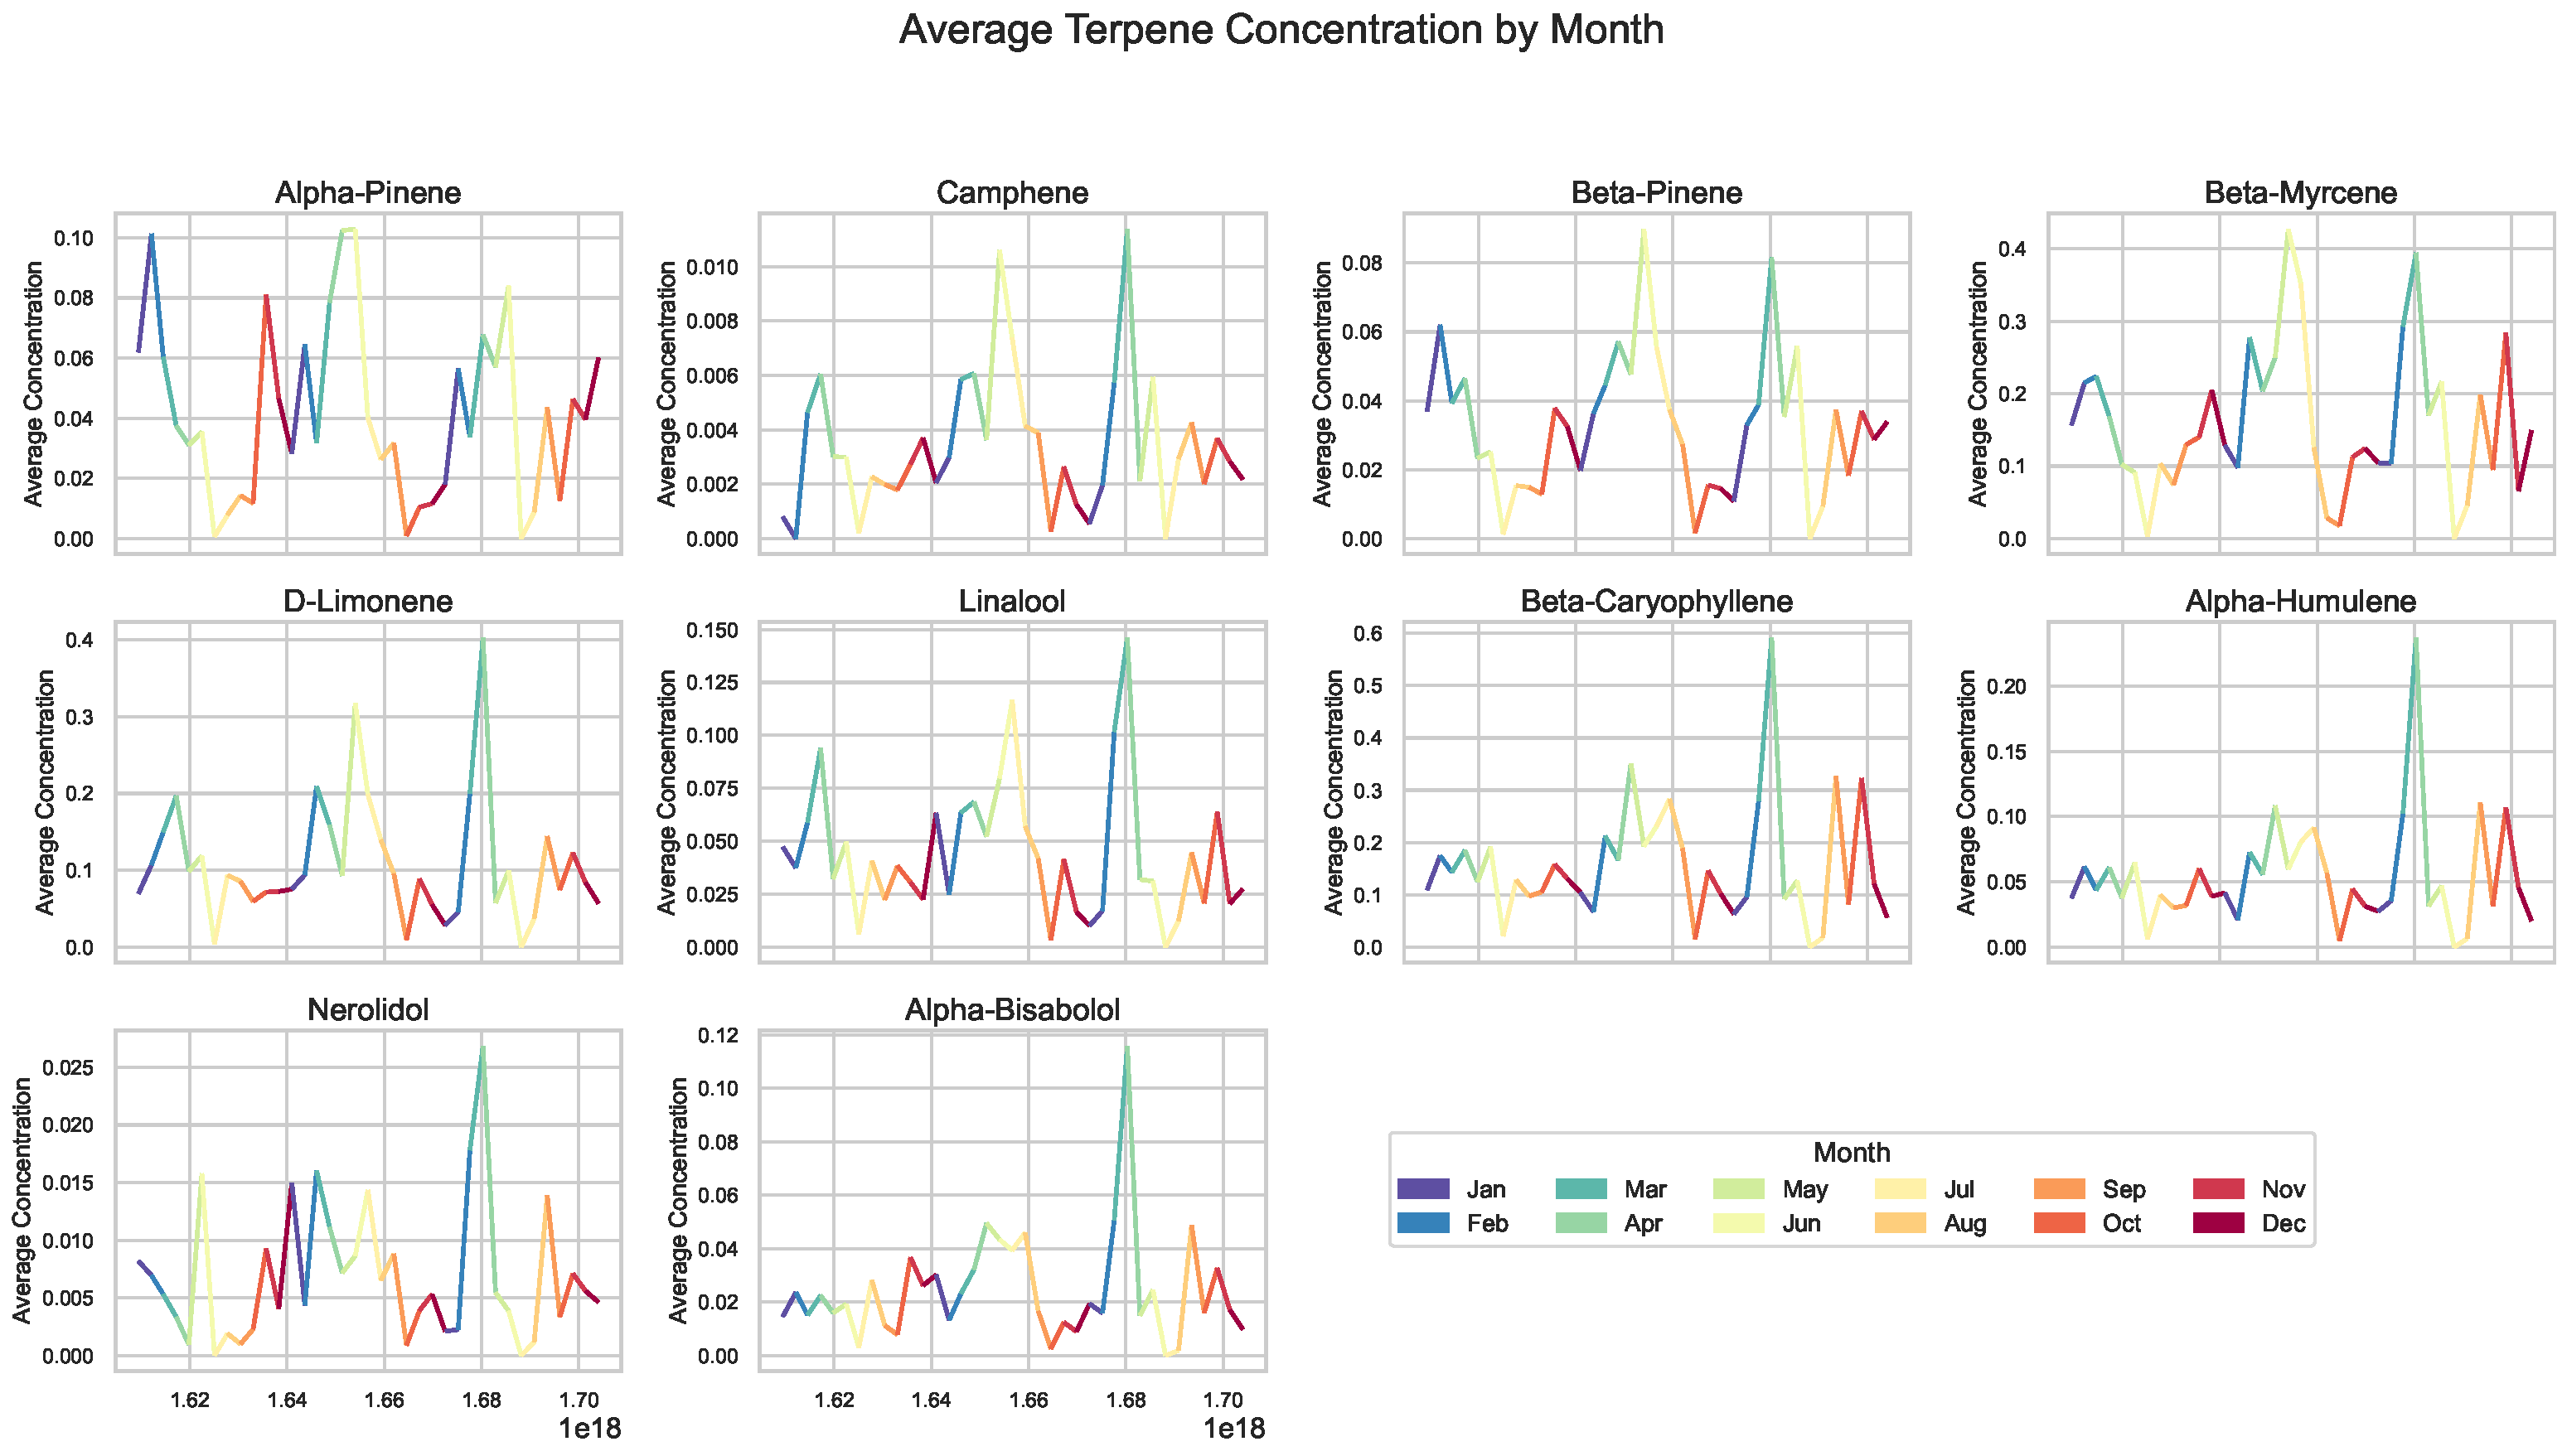
\includegraphics[width=\textwidth]{images/terpenes-by-month.pdf}
\end{center}
\end{frame}

% total-terpenes-by-zone
\begin{frame}{}
\begin{center}
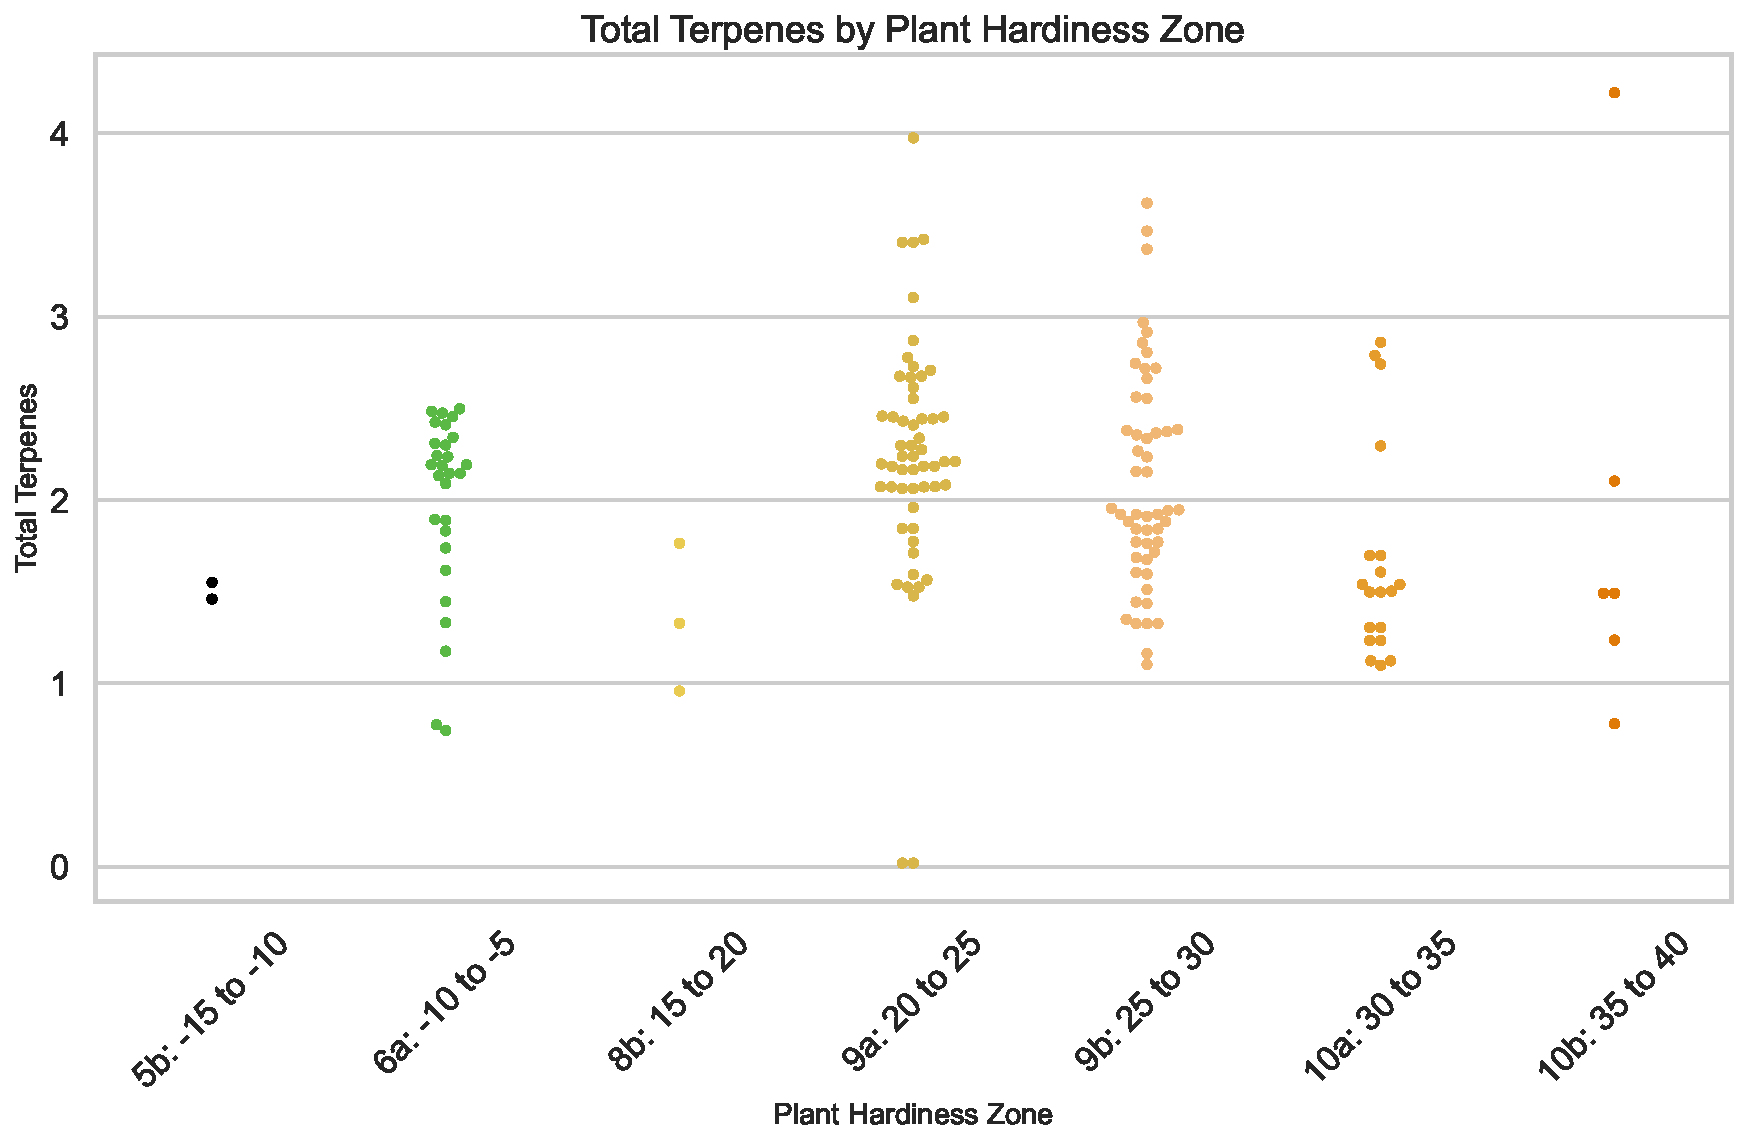
\includegraphics[width=\textwidth]{images/total-terpenes-by-zone.pdf}
\end{center}
\end{frame}

% terpenes-by-zone
\begin{frame}{}
\begin{center}
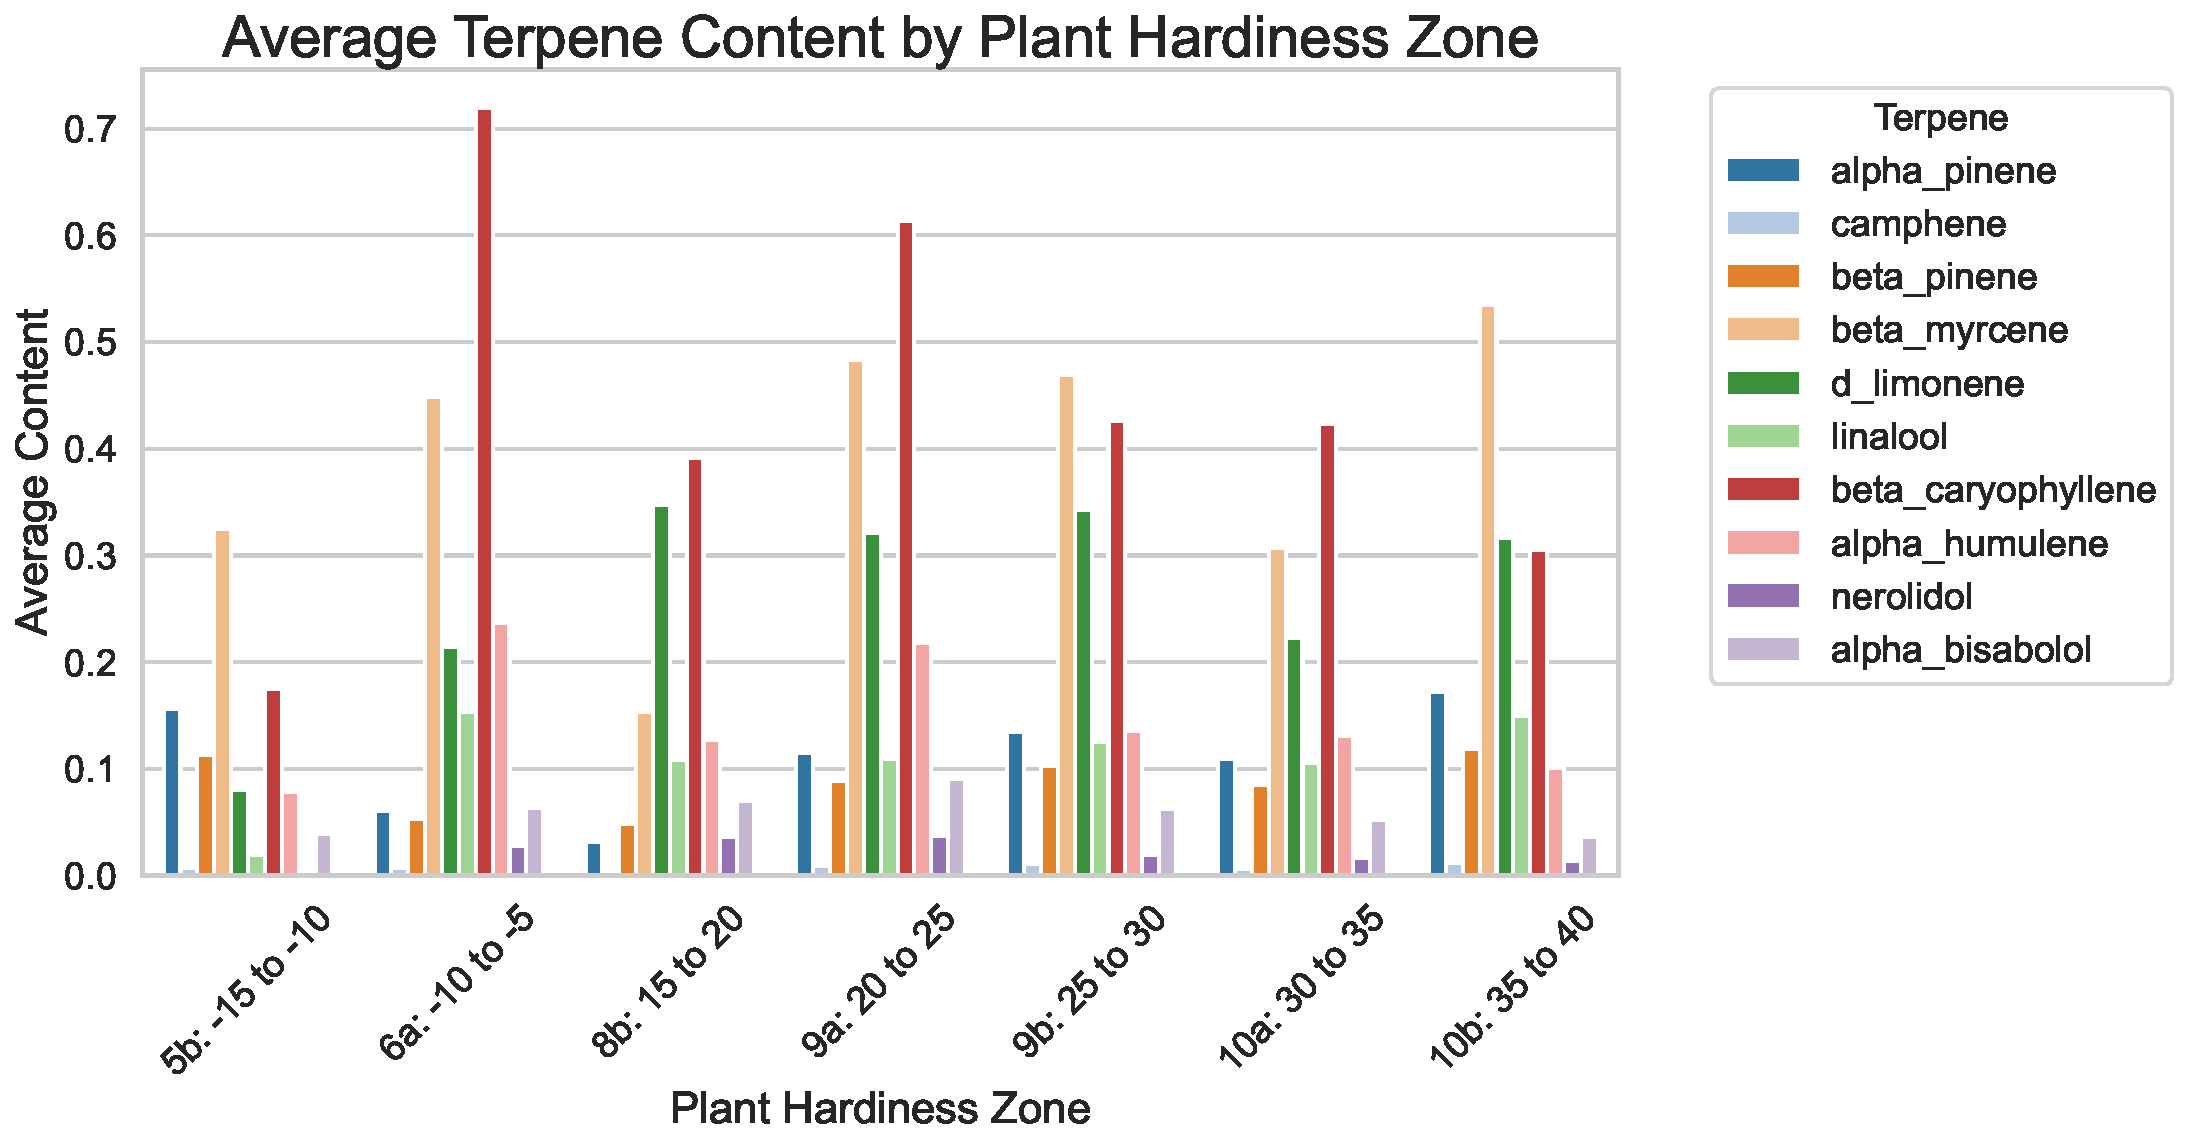
\includegraphics[width=\textwidth]{images/terpenes-by-zone.pdf}
\end{center}
\end{frame}



%------------------------------------------%
% Takeaway
%------------------------------------------%
\section{Takeaway}
\begin{frame}{}
\begin{center}
\begin{minipage}{3.85in}

\includegraphics[width=.25in]{images/prayer.png} {\Large \textbf{Thank you for coming.}}\\
\begin{center}
\begin{minipage}{\linewidth}
\begin{Block}{Lesson of the Day}
\vspace{\baselineskip}
\begin{itemize}

\item Always look on the bright side of life.
\vspace{\baselineskip}

\end{itemize}
\end{Block}
\end{minipage}
\end{center}
\vfill
\end{minipage}
\end{center}
\end{frame}

%------------------------------------------%
% End
%------------------------------------------%
\end{document}
